\begin{figure}[ht!]
  \centering
  \caption{Average marginal effects (logit-models)}\label{fig:Logit_ME}
  \begin{subfigure}[b]{\textwidth}
  \centering
  \caption{Average marginal effects of total household expenditures (log)} \label{fig:Logit_ME_exp}
  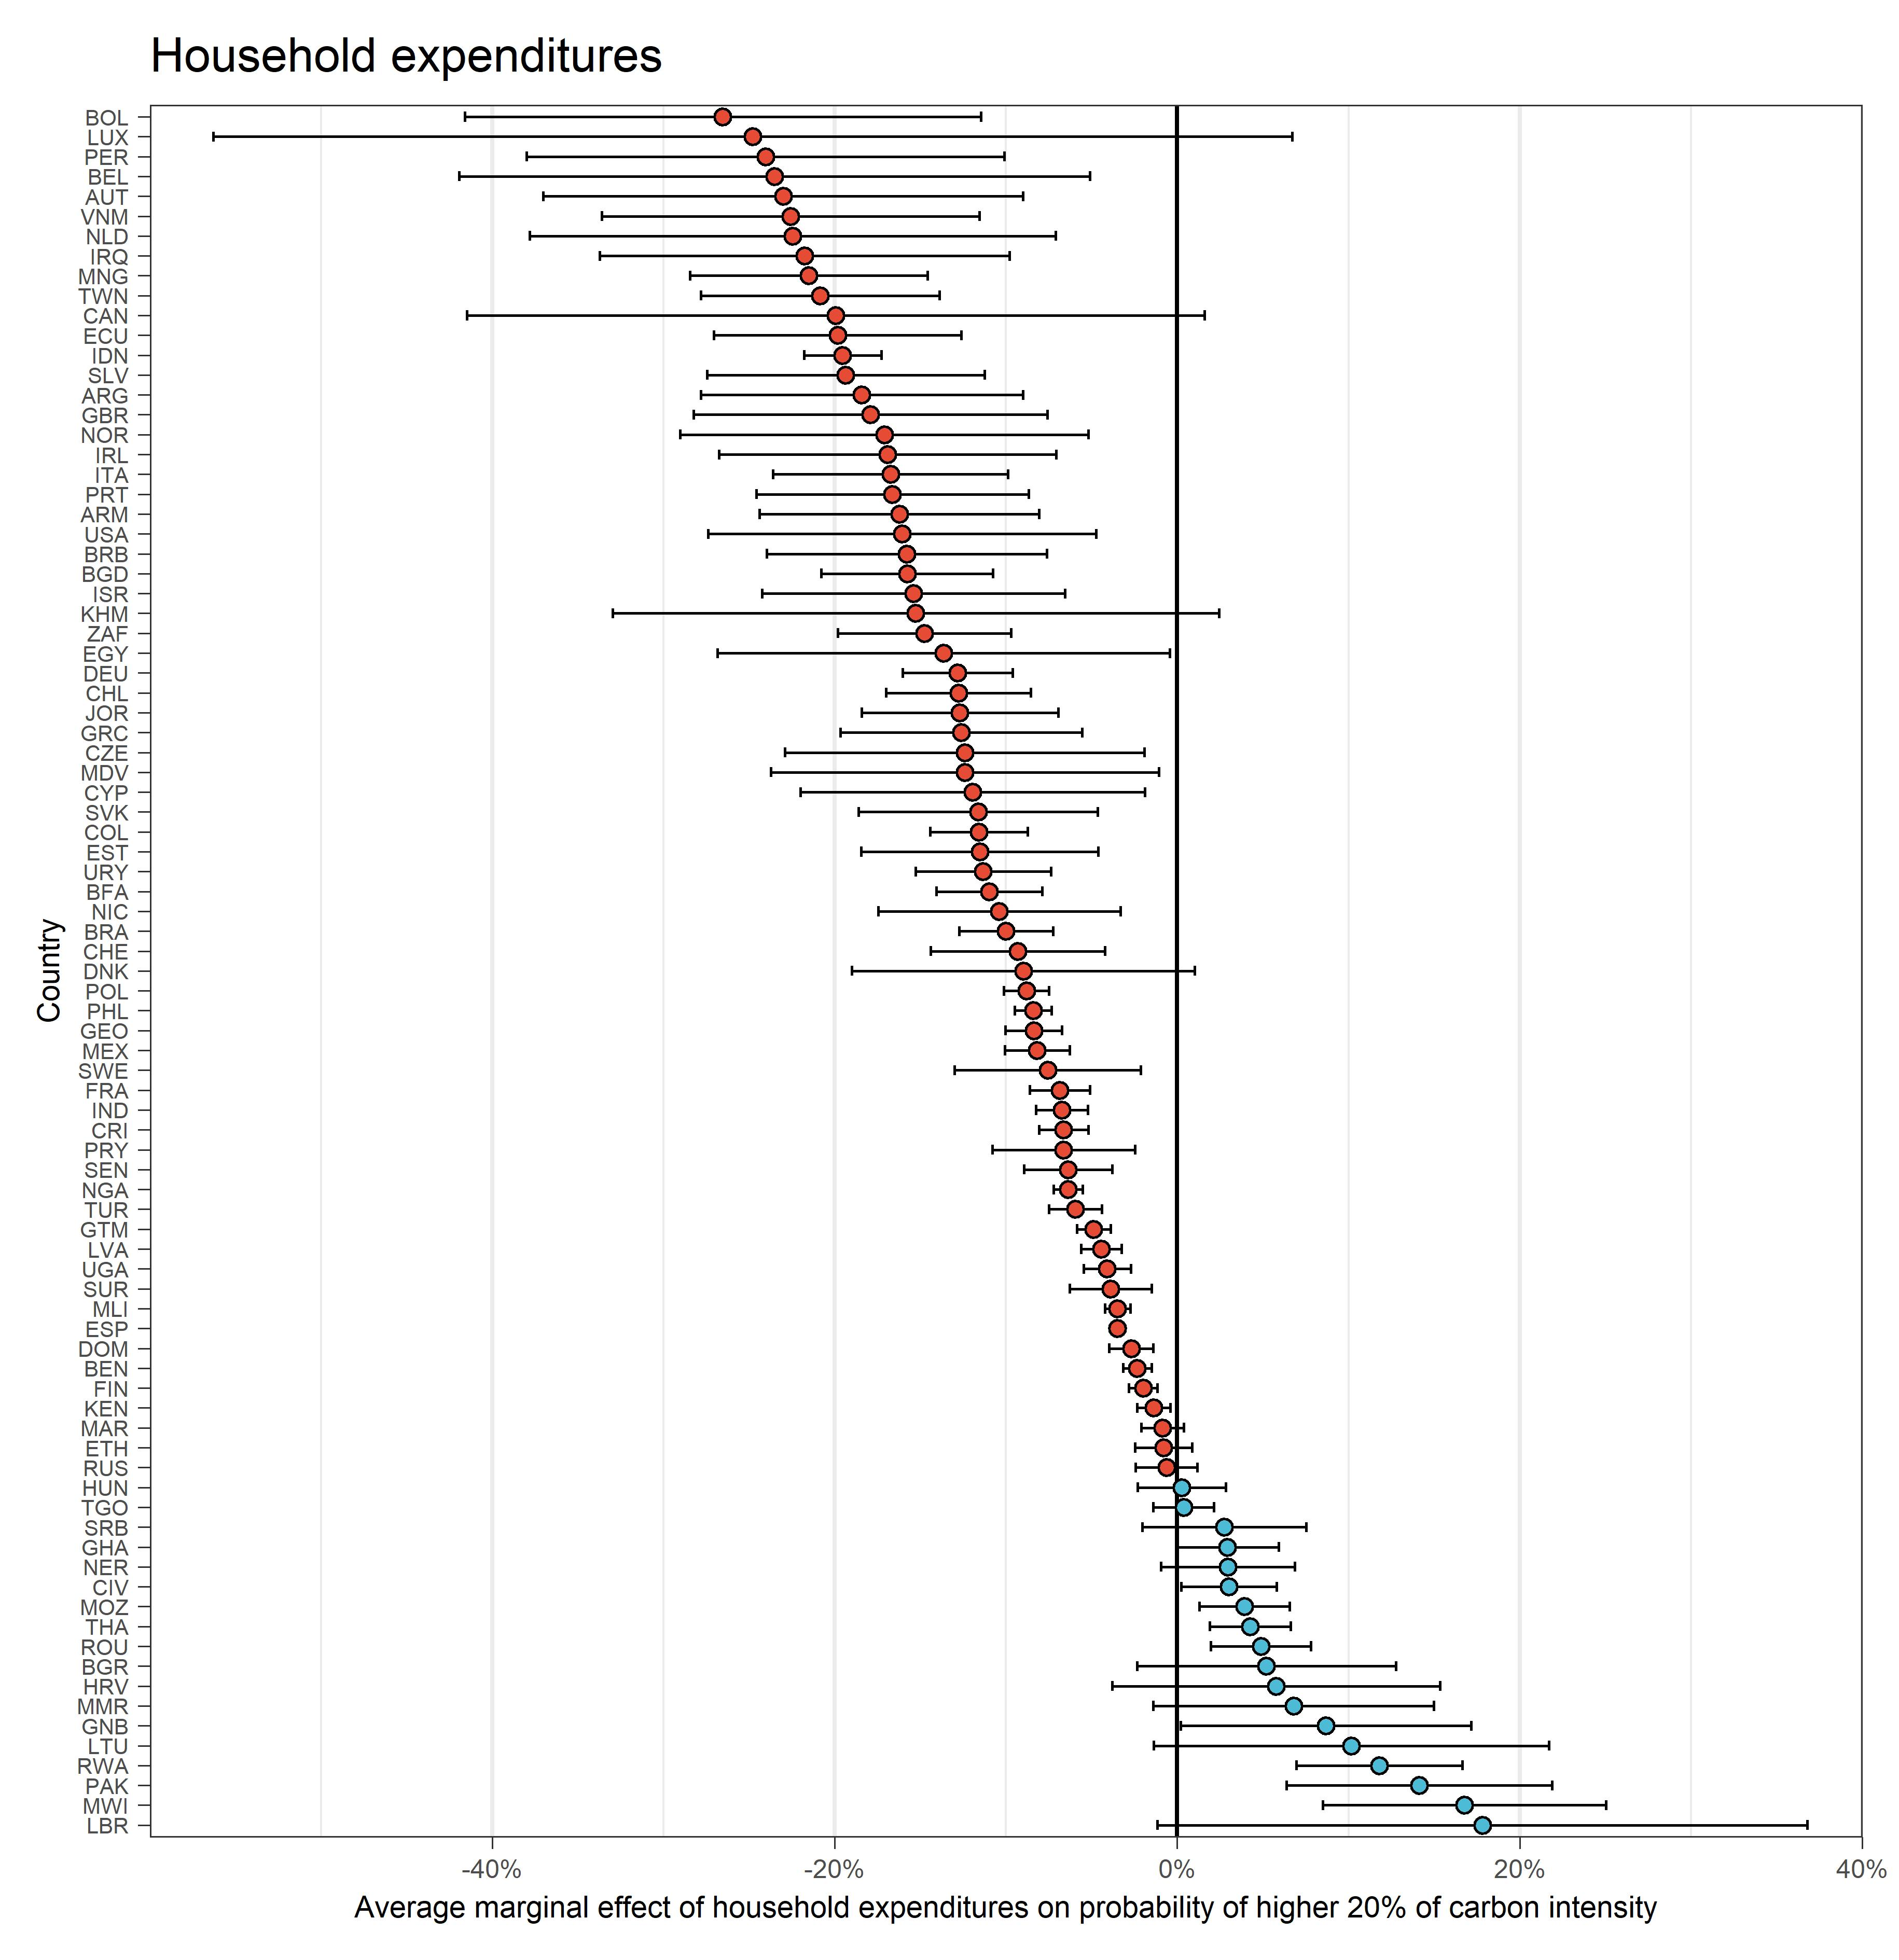
\includegraphics{1_Figures/Analysis_Logit_Models_Marginal_Effects/Average_Marginal_Effects_affected_upper_80_log_hh_expenditures_USD_2014_2017.jpg}
  \begin{subcaption2}
     This figure shows average marginal effects of 1\% increase in total household expenditures on the probability of consuming more carbon intensively than 80\% of households in each country. Estimates come from logit-models (see equation \ref{logit}) including a rich set of control variables. Control variables differ for different countries. Red points display negative estimates; blue points display positive estimates. Error bars display 95\%-confidence interval. Estimates are ordered in descending order.
  \end{subcaption2}
  \end{subfigure}
 \end{figure}
 \clearpage

 \begin{figure}[ht!]\ContinuedFloat
   \centering
   \begin{subfigure}[b]{\textwidth}
   \centering
   \caption{Average marginal effects of household size} \label{fig:Logit_ME_size}
   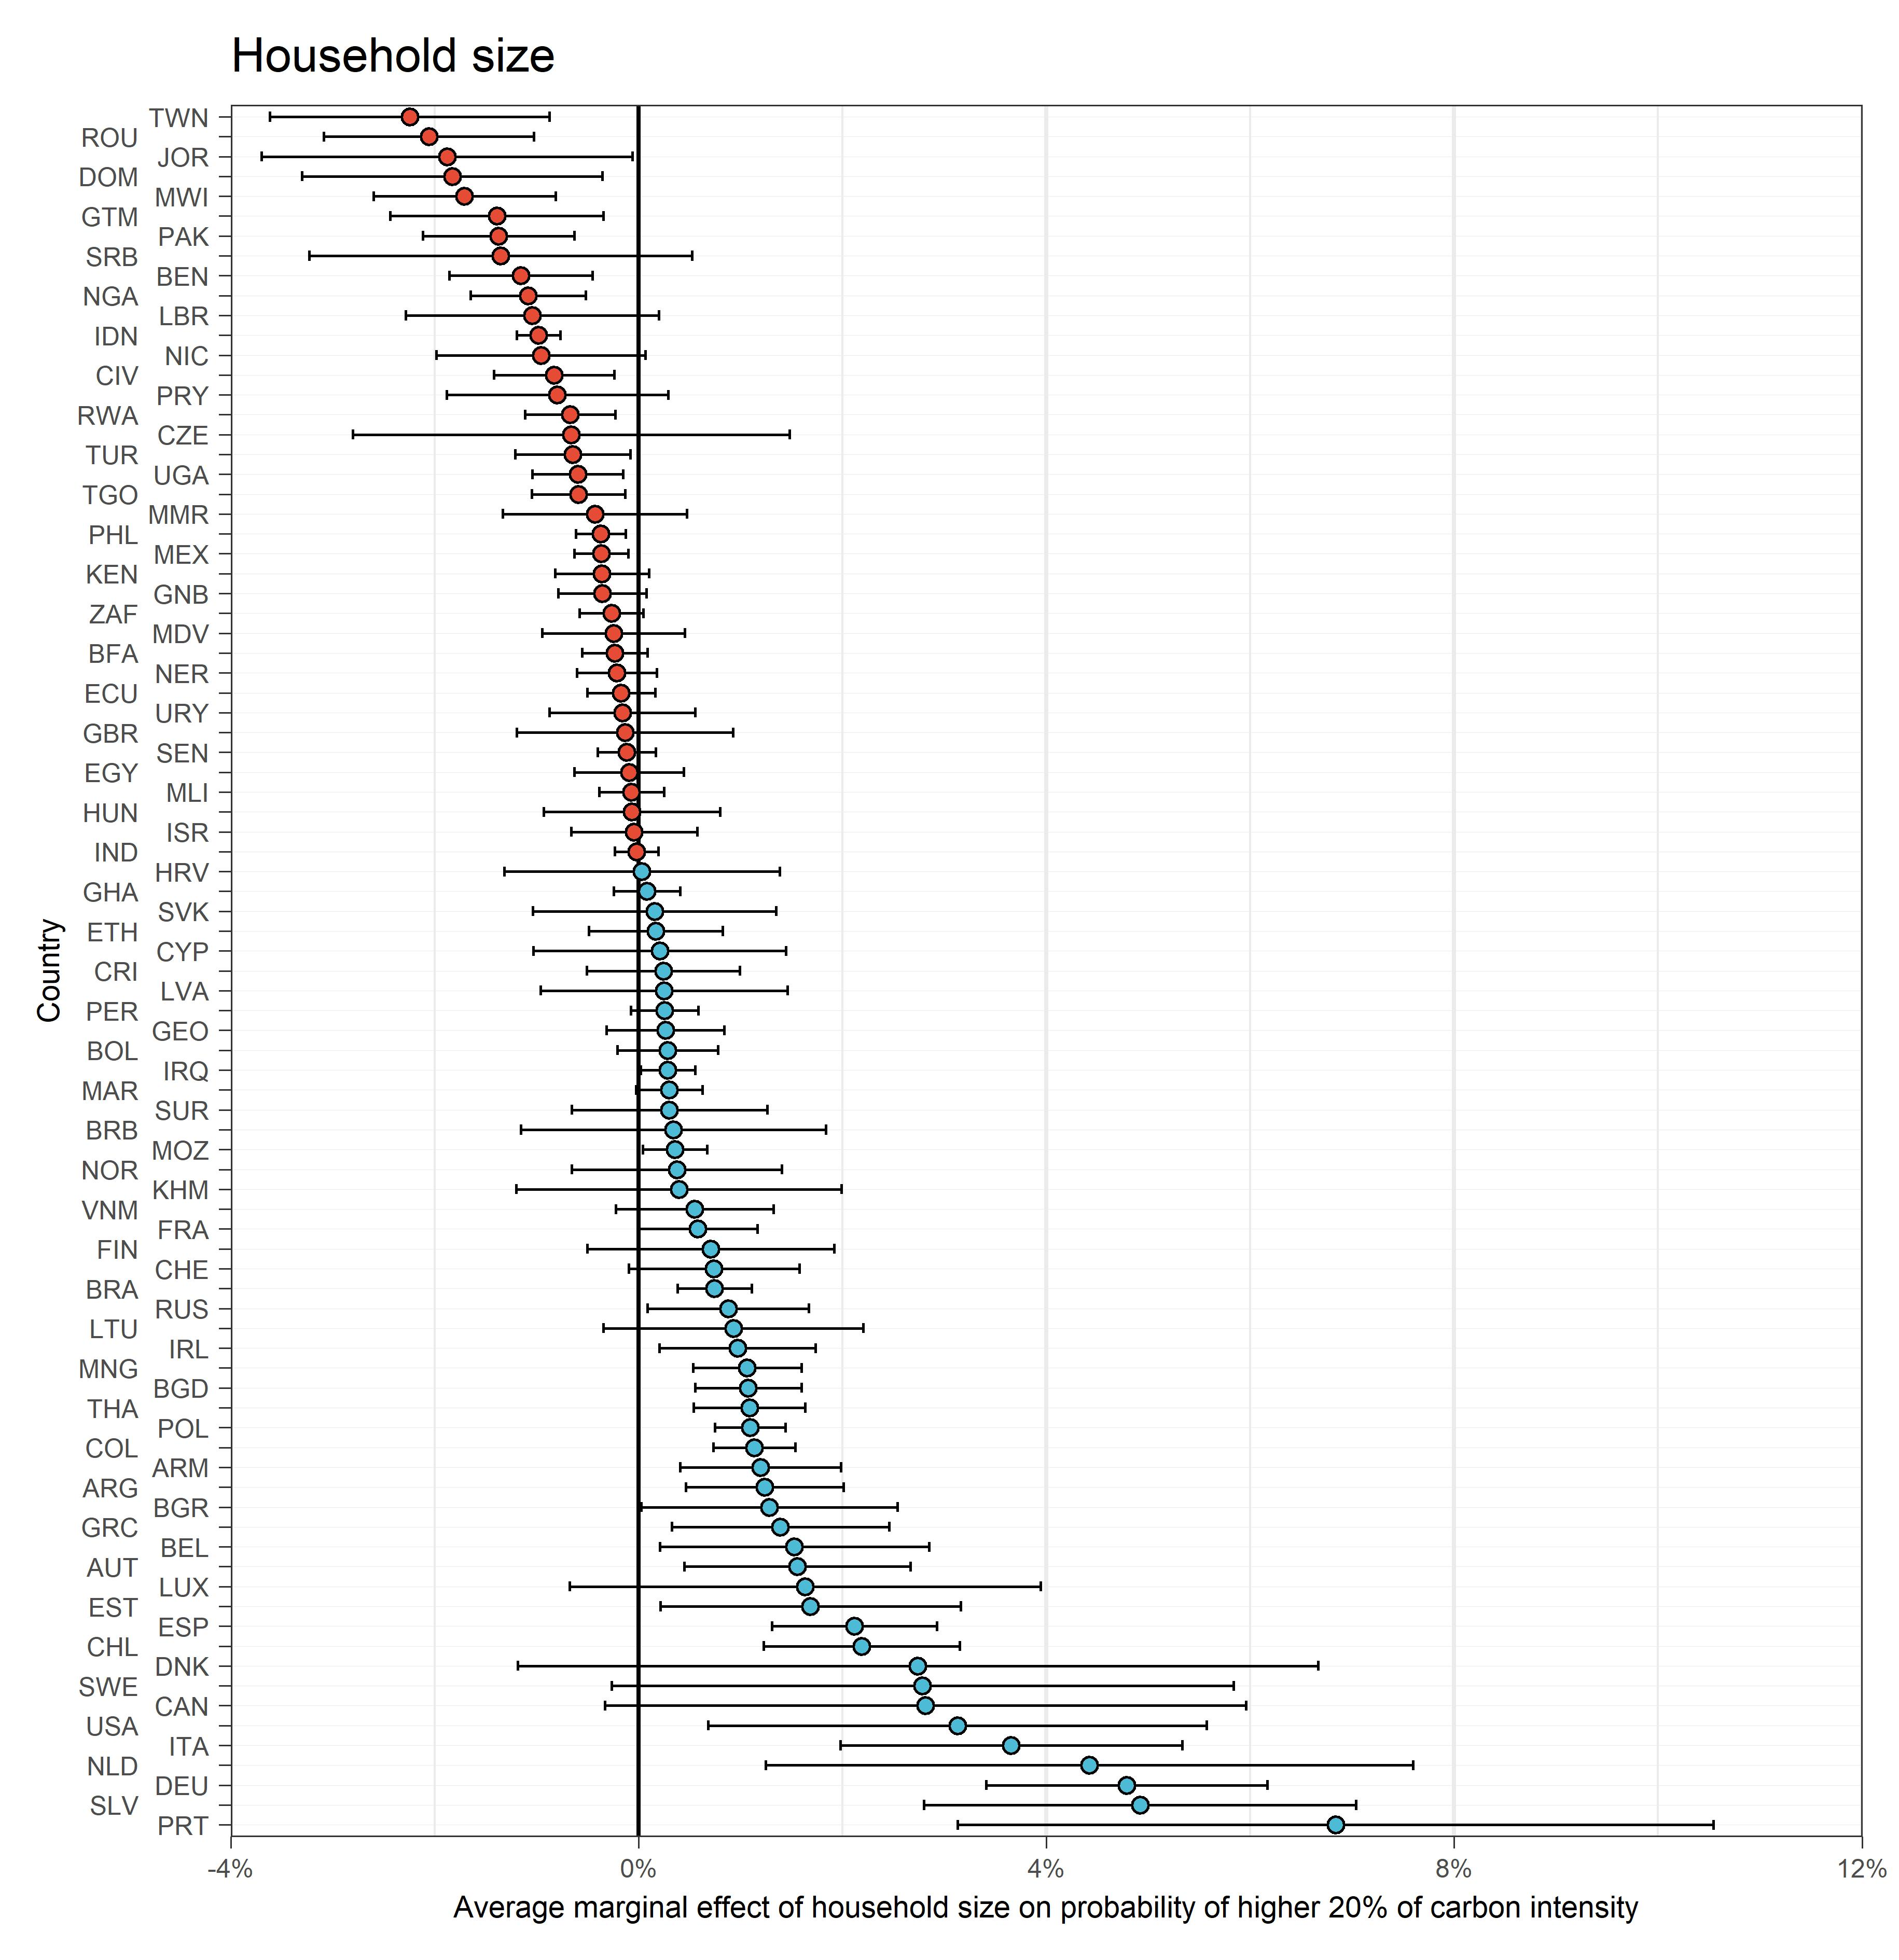
\includegraphics{1_Figures/Analysis_Logit_Models_Marginal_Effects/Average_Marginal_Effects_affected_upper_80_hh_size_2017.jpg}
   \begin{subcaption2}
     This figure shows average marginal effects of household size on the probability of consuming more carbon intensively than 80\% of households in each country. Estimates come from logit-models (see equation \ref{logit}) including a rich set of control variables including total household expenditures. Control variables differ for different countries. Red points display negative estimates; blue points display positive estimates. Error bars display 95\%-confidence interval. Estimates are ordered in descending order.
   \end{subcaption2}
   \end{subfigure}
 \end{figure}
 \clearpage

 \begin{figure}[ht!]\ContinuedFloat
   \centering
   \begin{subfigure}[b]{\textwidth}
   \centering
   \caption{Average marginal effects of urban citizenship} \label{fig:Logit_ME_urban}
   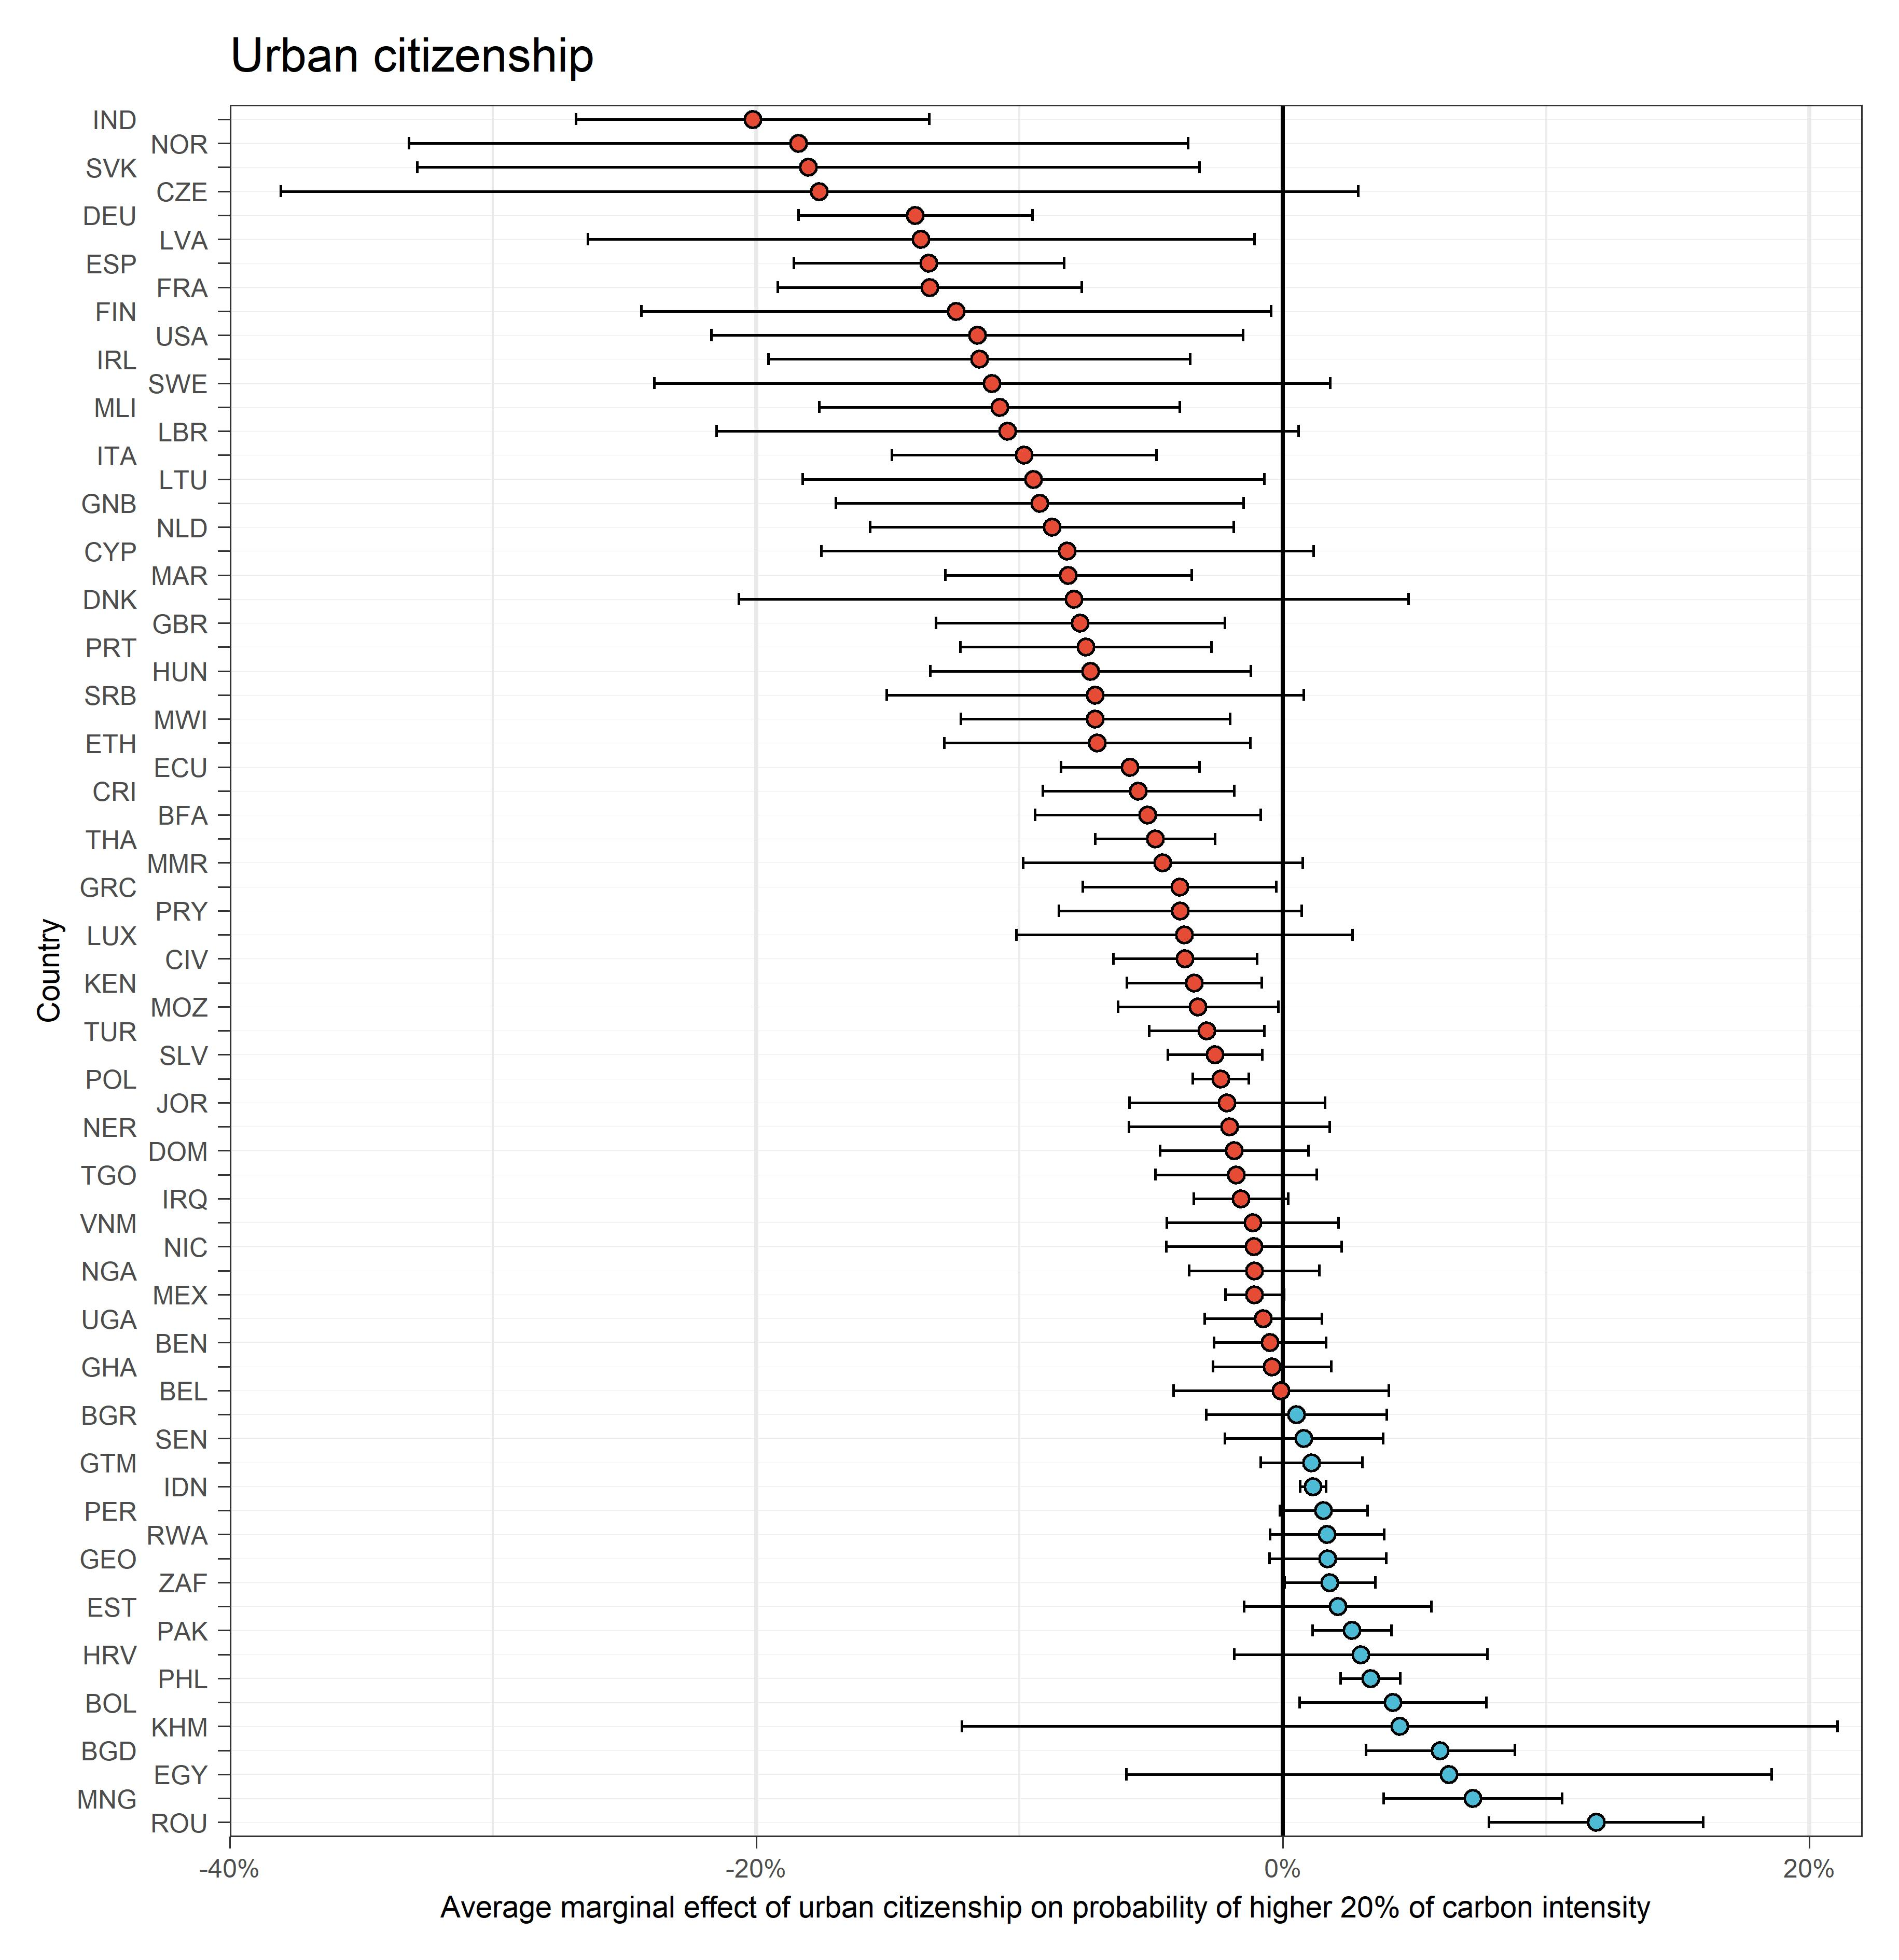
\includegraphics{1_Figures/Analysis_Logit_Models_Marginal_Effects/Average_Marginal_Effects_affected_upper_80_urban_01_2017.jpg}
   \begin{subcaption2}
     This figure shows average marginal effects of urban citizenship (in contrast to rural citizenship) on the probability of consuming more carbon intensively than 80\% of households in each country. Estimates come from logit-models (see equation \ref{logit}) including a rich set of control variables including total household expenditures. Control variables differ for different countries. Red points display negative estimates; blue points display positive estimates. Error bars display 95\%-confidence interval. Estimates are ordered in descending order.
   \end{subcaption2}
   \end{subfigure}
 \end{figure}
 \clearpage

 \begin{figure}[ht!]\ContinuedFloat
   \centering
   \begin{subfigure}[b]{\textwidth}
   \centering
   \caption{Average marginal effects of car ownership} \label{fig:Logit_ME_car}
   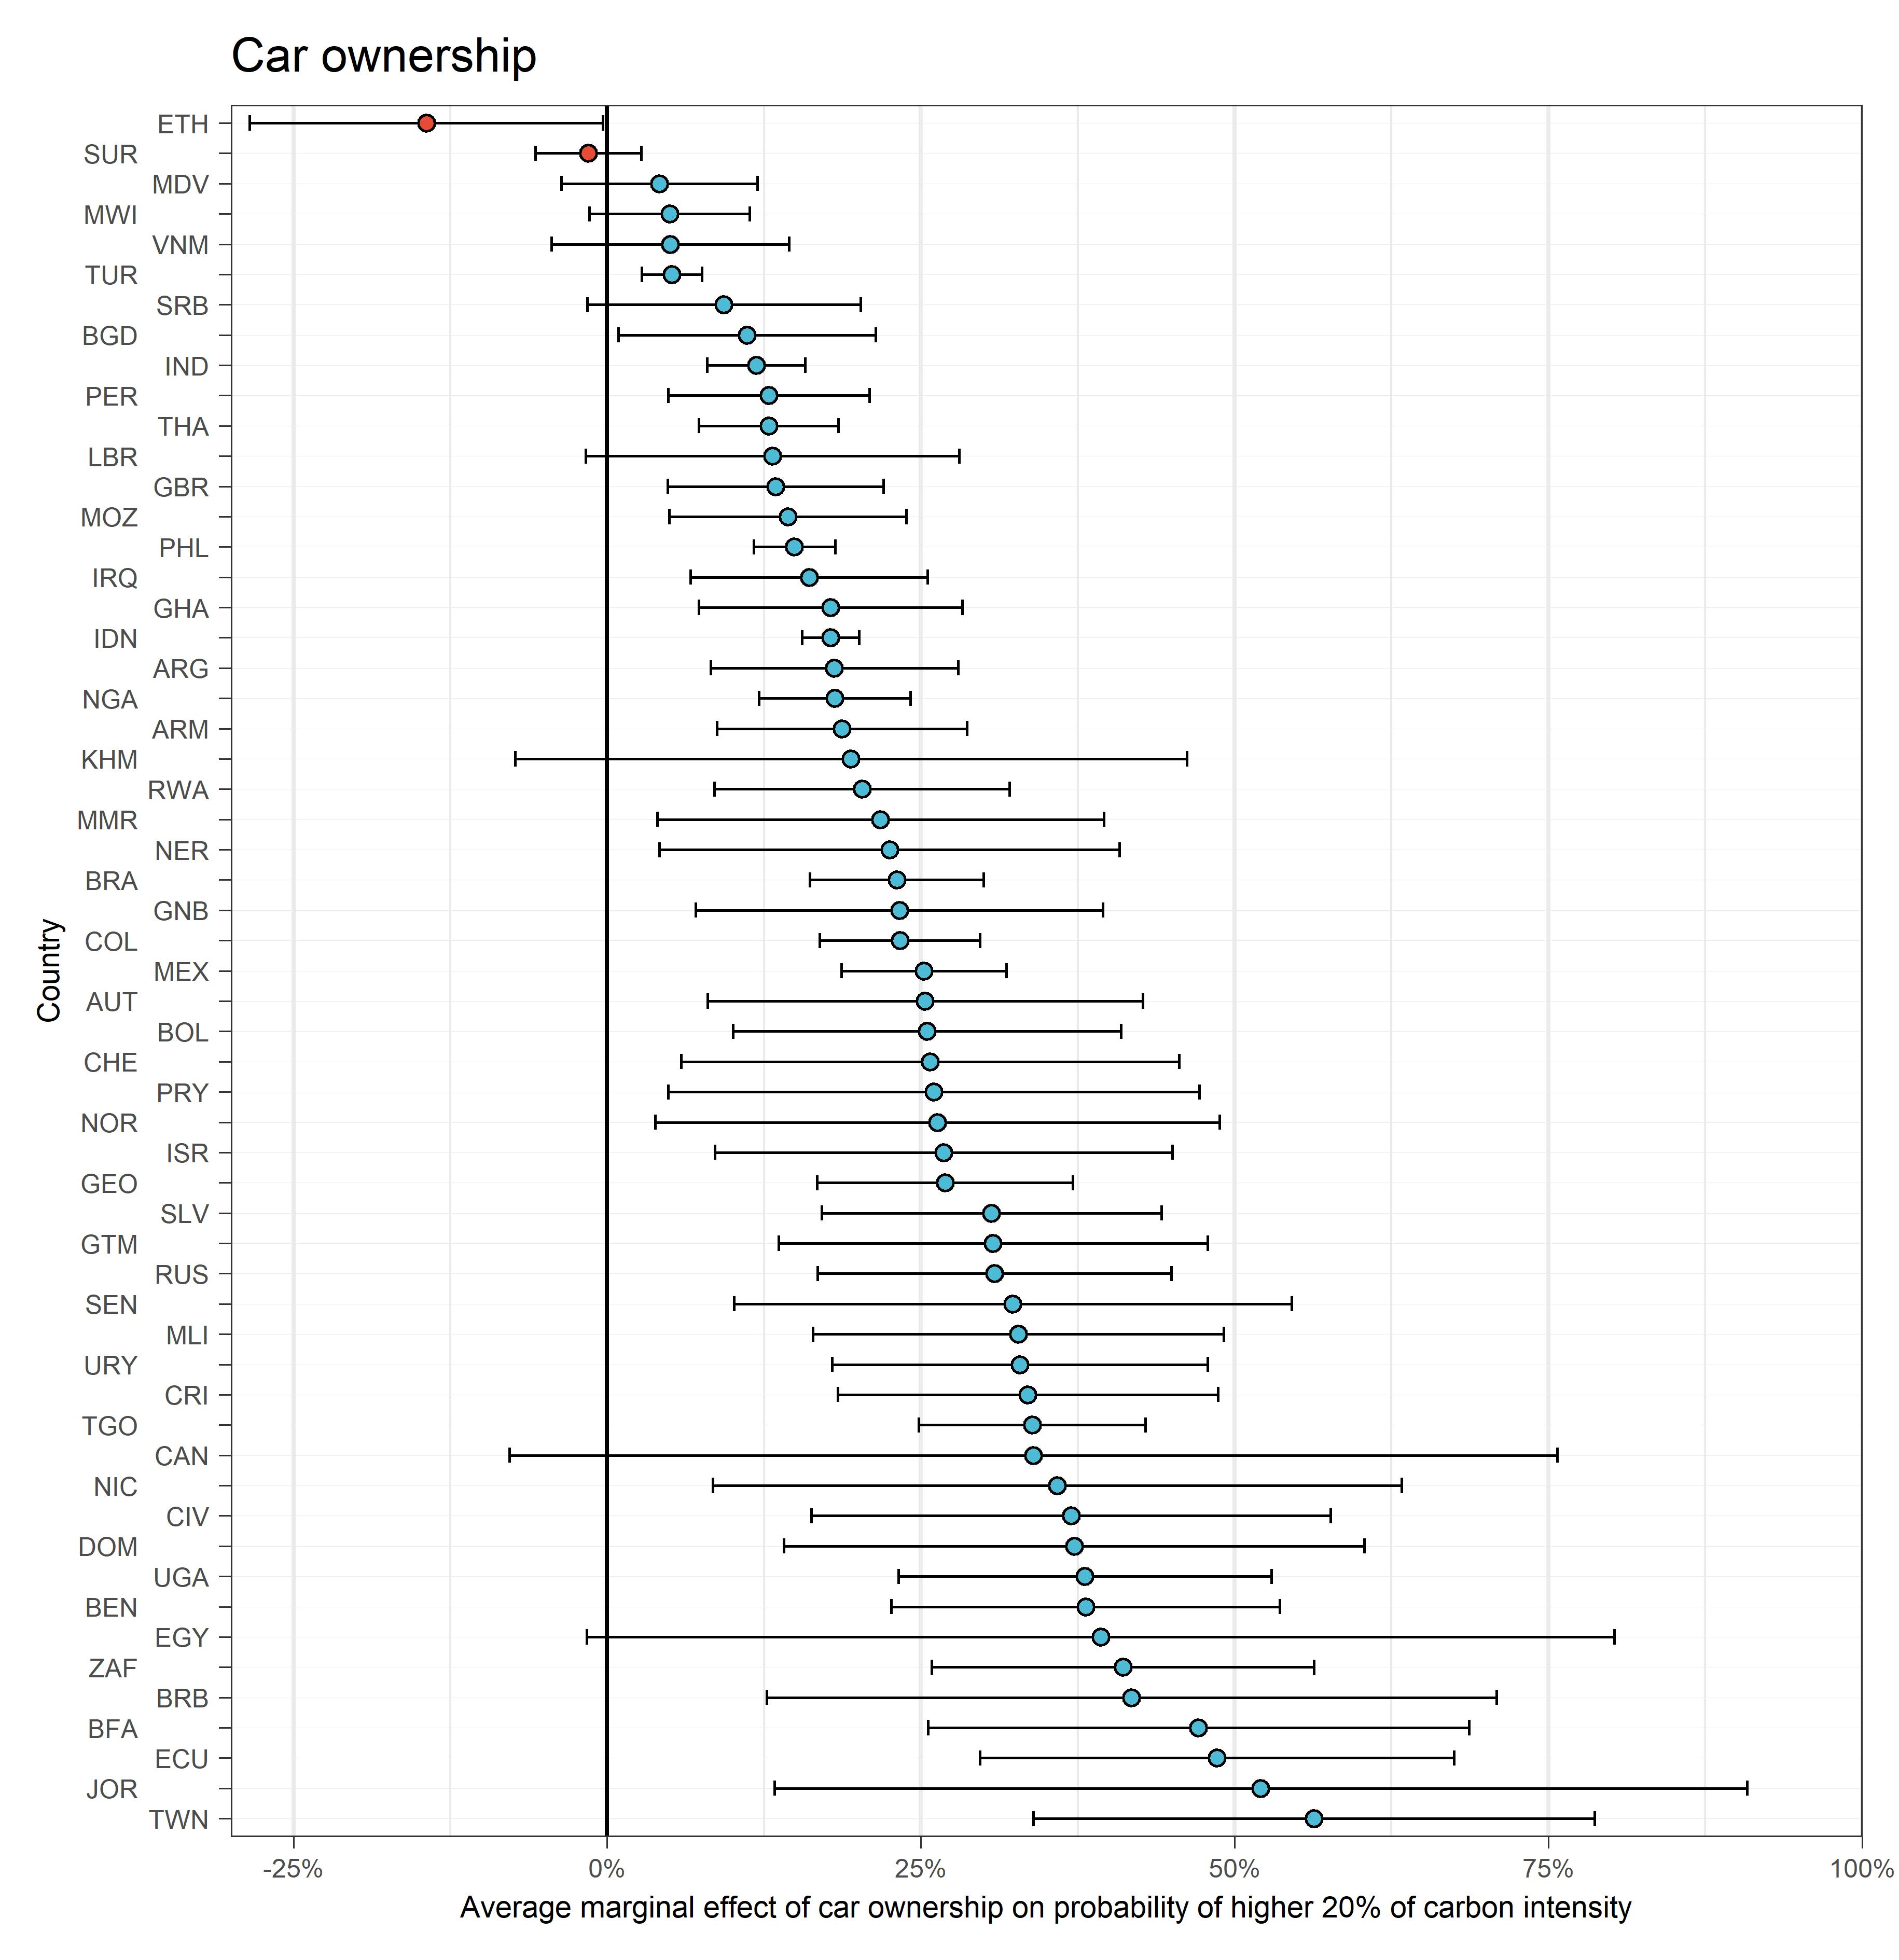
\includegraphics{1_Figures/Analysis_Logit_Models_Marginal_Effects/Average_Marginal_Effects_affected_upper_80_car.01_2017.jpg}
   \begin{subcaption2}
     This figure shows average marginal effects of car ownership on the probability of consuming more carbon intensively than 80\% of households in each country. Estimates come from logit-models (see equation \ref{logit}) including a rich set of control variables including total household expenditures. Control variables differ for different countries. Red points display negative estimates; blue points display positive estimates. Error bars display 95\%-confidence interval. Estimates are ordered in descending order.
   \end{subcaption2}
   \end{subfigure}
 \end{figure}
 \clearpage

 \begin{figure}[ht!]\ContinuedFloat
   \centering
   \begin{subfigure}[b]{\textwidth}
   \centering
   \caption{Average marginal effects of motorcycle ownership} \label{fig:Logit_ME_motorcycle}
   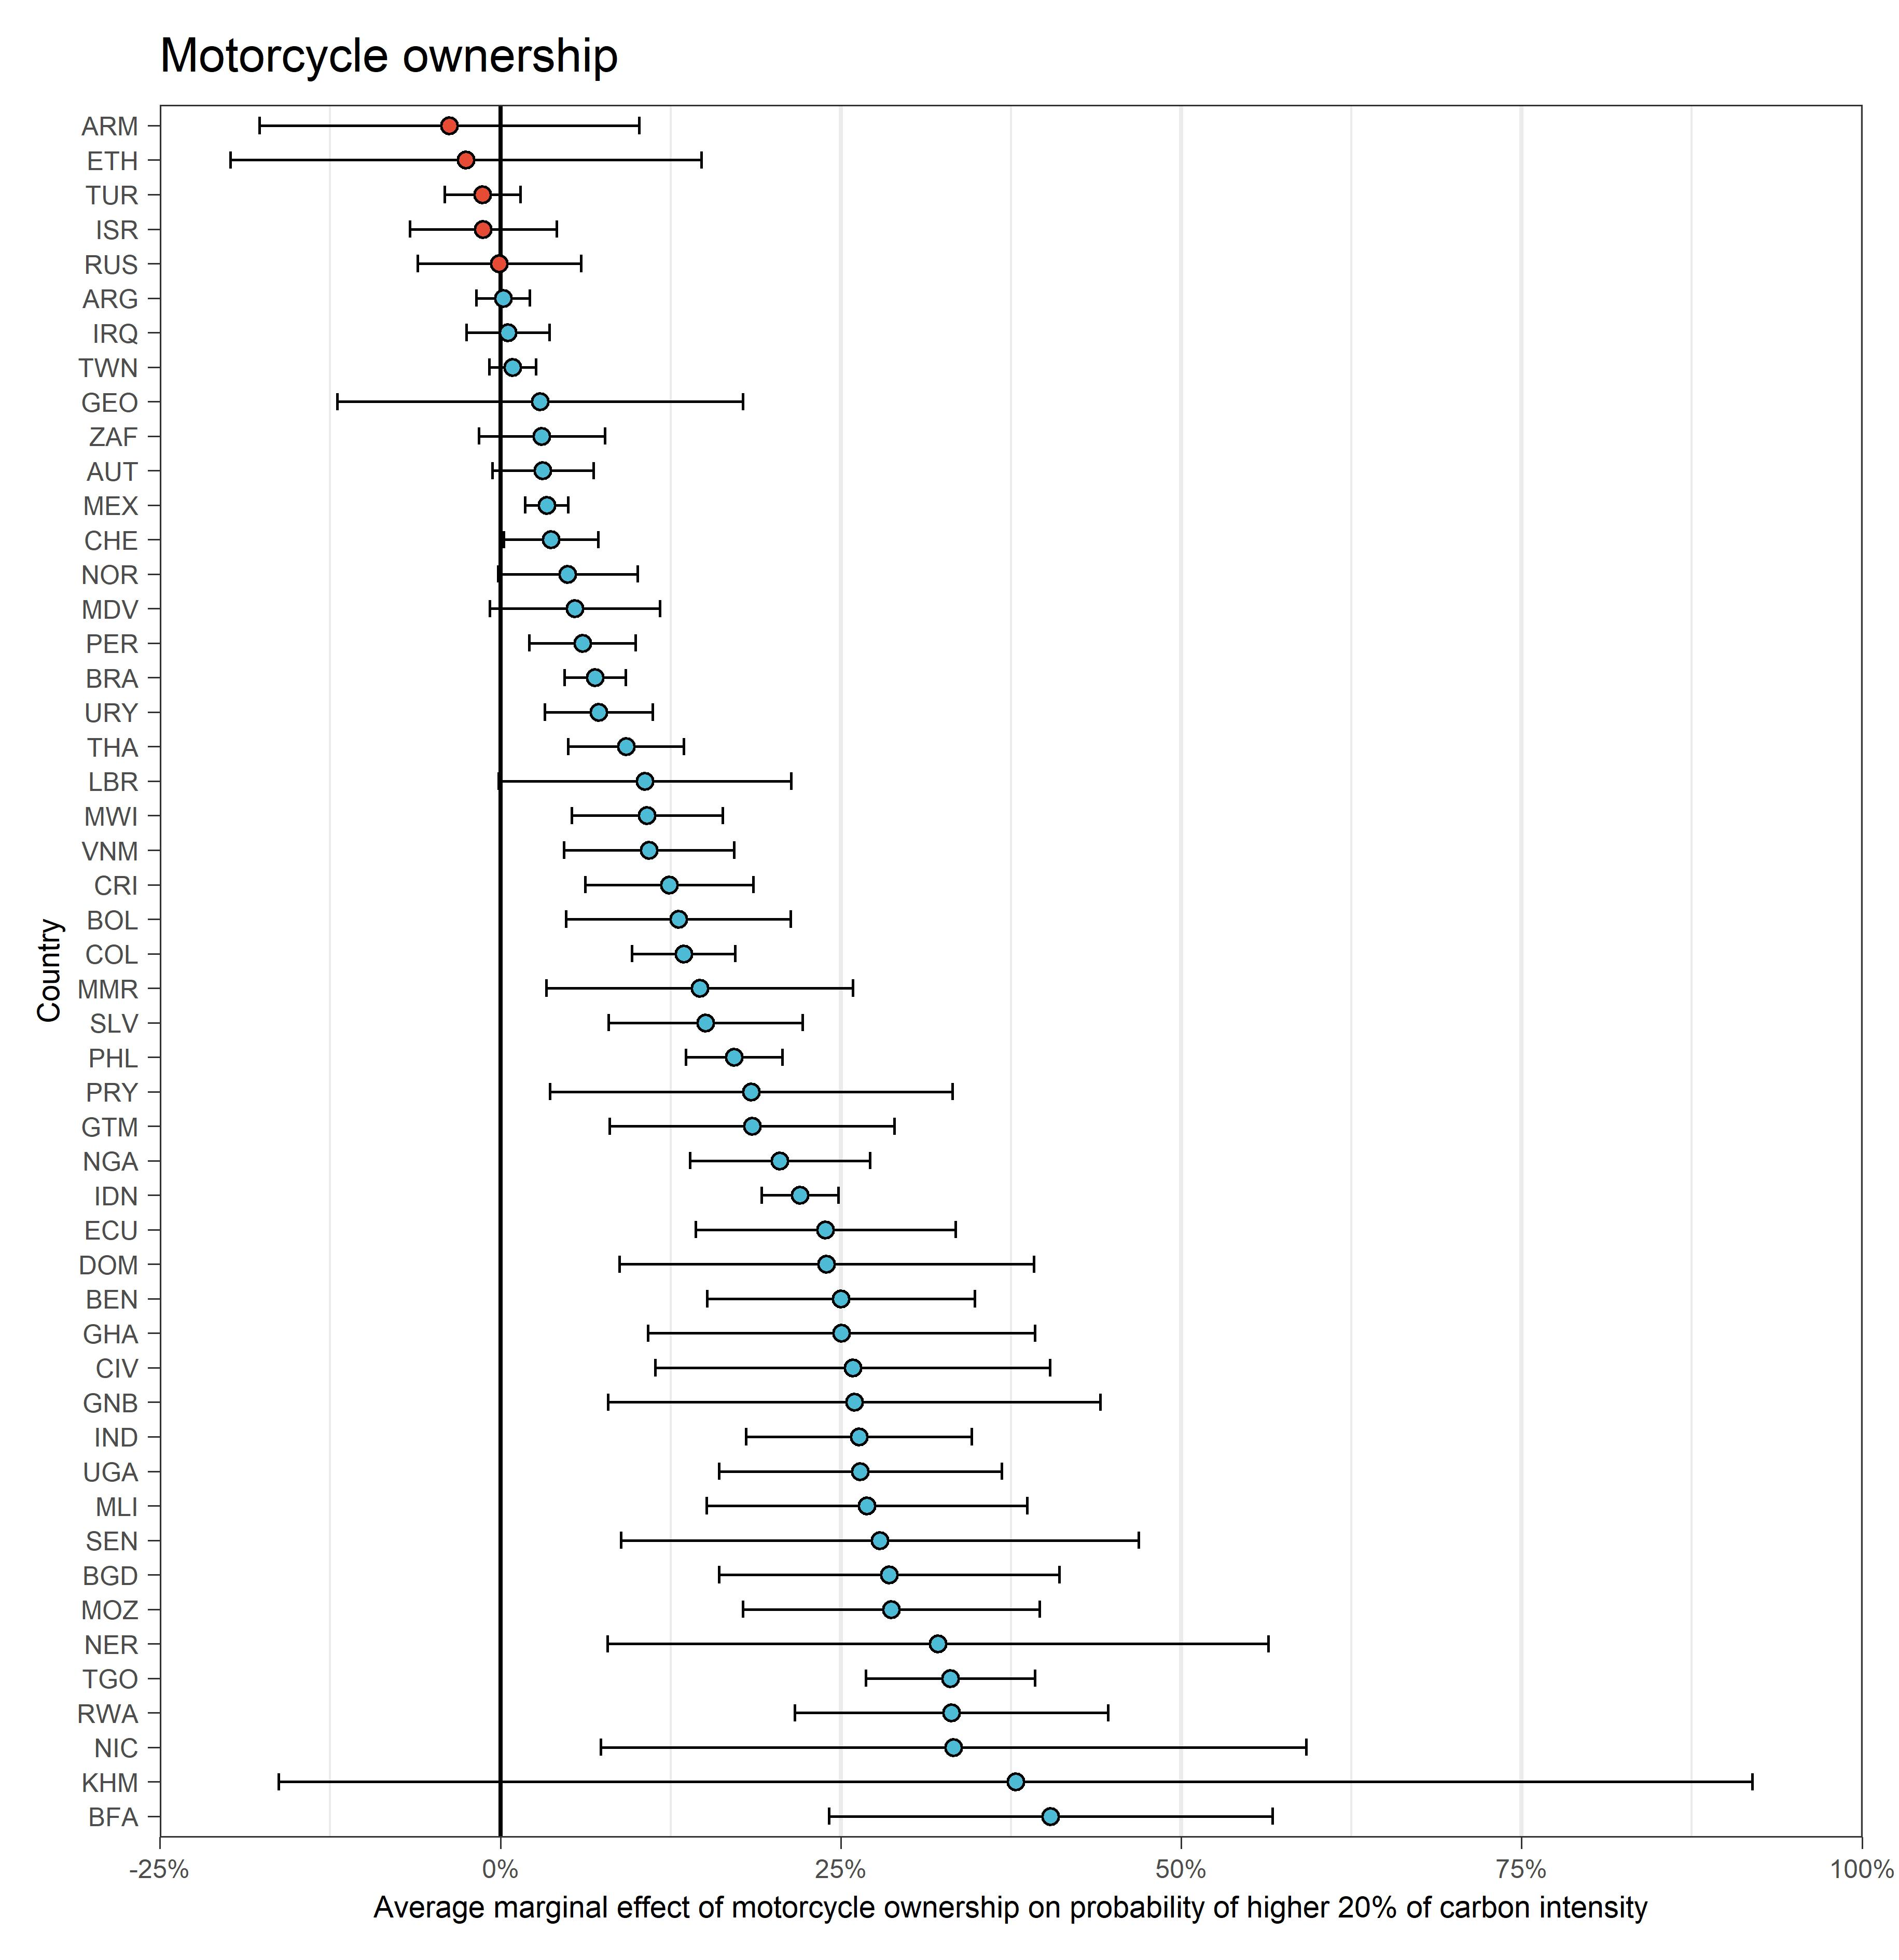
\includegraphics{1_Figures/Analysis_Logit_Models_Marginal_Effects/Average_Marginal_Effects_affected_upper_80_motorcycle.01_2017.jpg}
   \begin{subcaption2}
     This figure shows average marginal effects of motorcycle ownership on the probability of consuming more carbon intensively than 80\% of households in each country. Estimates come from logit-models (see equation \ref{logit}) including a rich set of control variables including total household expenditures. Control variables differ for different countries. Red points display negative estimates; blue points display positive estimates. Error bars display 95\%-confidence interval. Estimates are ordered in descending order.
   \end{subcaption2}
   \end{subfigure}
 \end{figure}
 \clearpage

 \begin{figure}[ht!]\ContinuedFloat
   \centering
   \begin{subfigure}[b]{\textwidth}
   \centering
   \caption{Average marginal effects of electricity access} \label{fig:Logit_ME_electricity}
   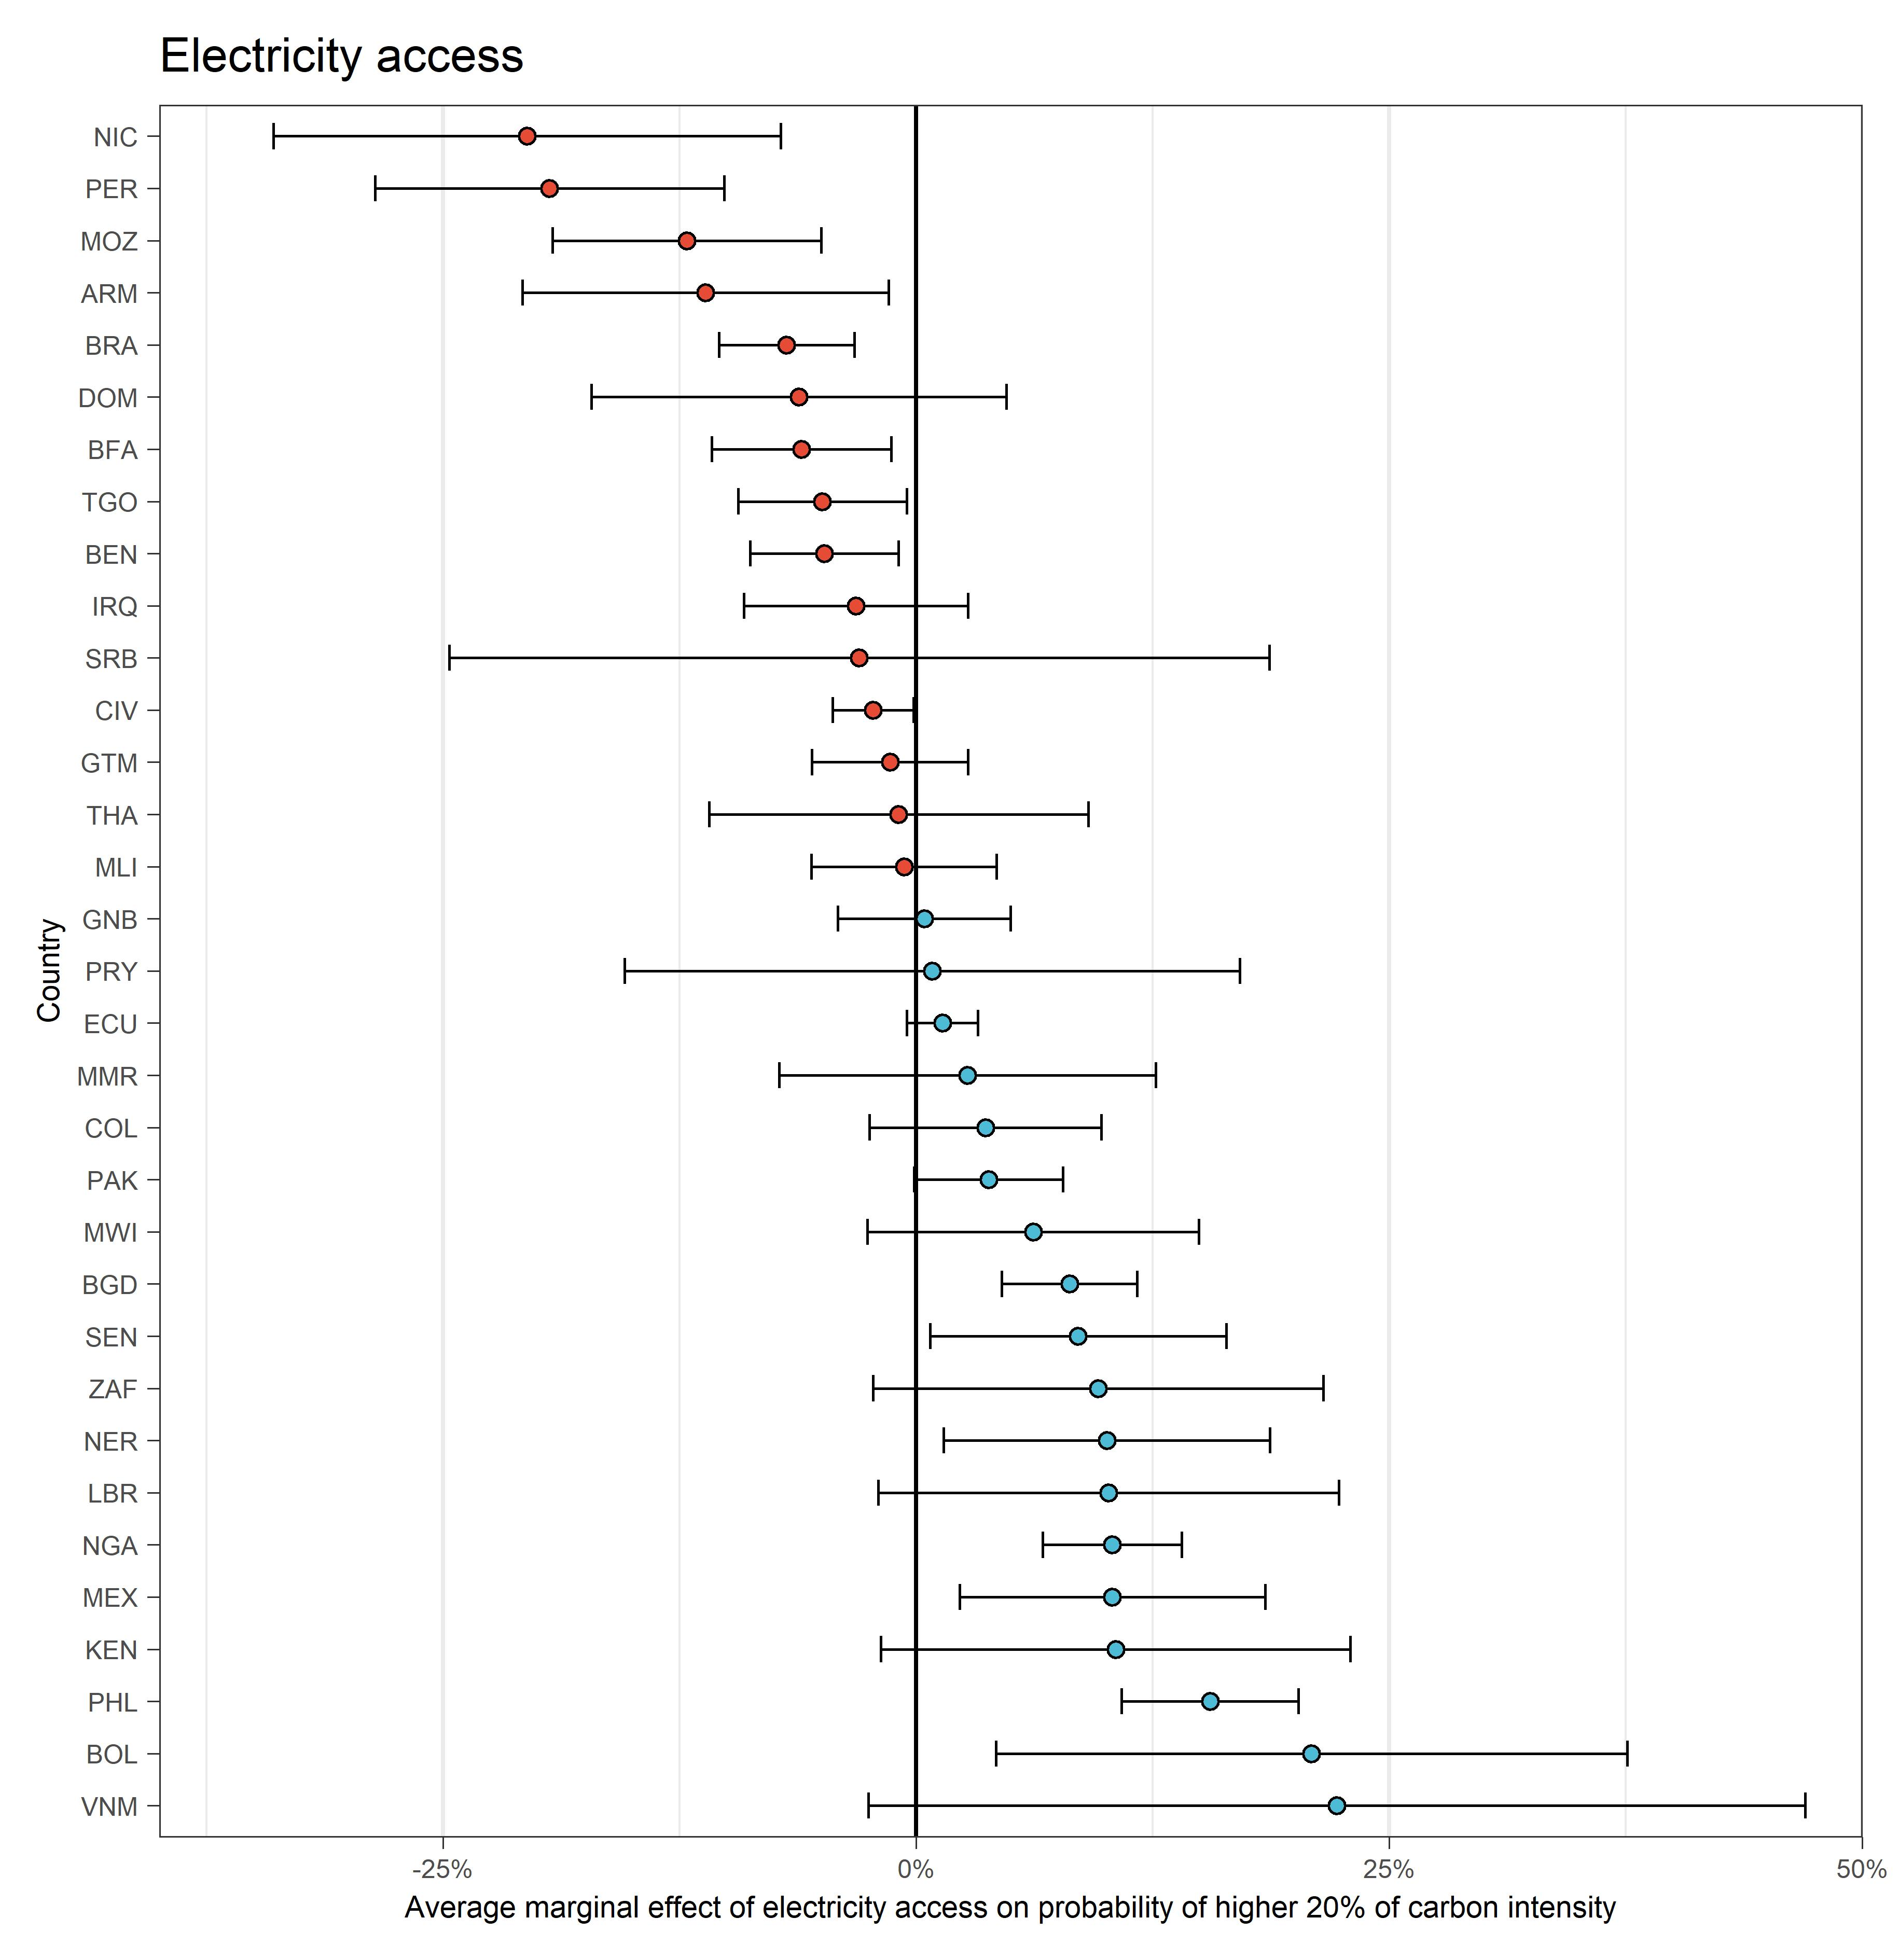
\includegraphics{1_Figures/Analysis_Logit_Models_Marginal_Effects/Average_Marginal_Effects_affected_upper_80_electricity.access_2017.jpg}
   \begin{subcaption2}
     This figure shows average marginal effects of electricity access on the probability of consuming more carbon intensively than 80\% of households in each country. Estimates come from logit-models (see equation \ref{logit}) including a rich set of control variables including total household expenditures. Control variables differ for different countries. Red points display negative estimates; blue points display positive estimates. Error bars display 95\%-confidence interval. Estimates are ordered in descending order.
   \end{subcaption2}
   \end{subfigure}
 \end{figure}
 \clearpage

 \begin{figure}[ht!]\ContinuedFloat
   \centering
   \begin{subfigure}[b]{\textwidth}
   \centering
   \caption{Average marginal effects of cooking fuel choice - part A} \label{fig:Logit_ME_CF_1}
   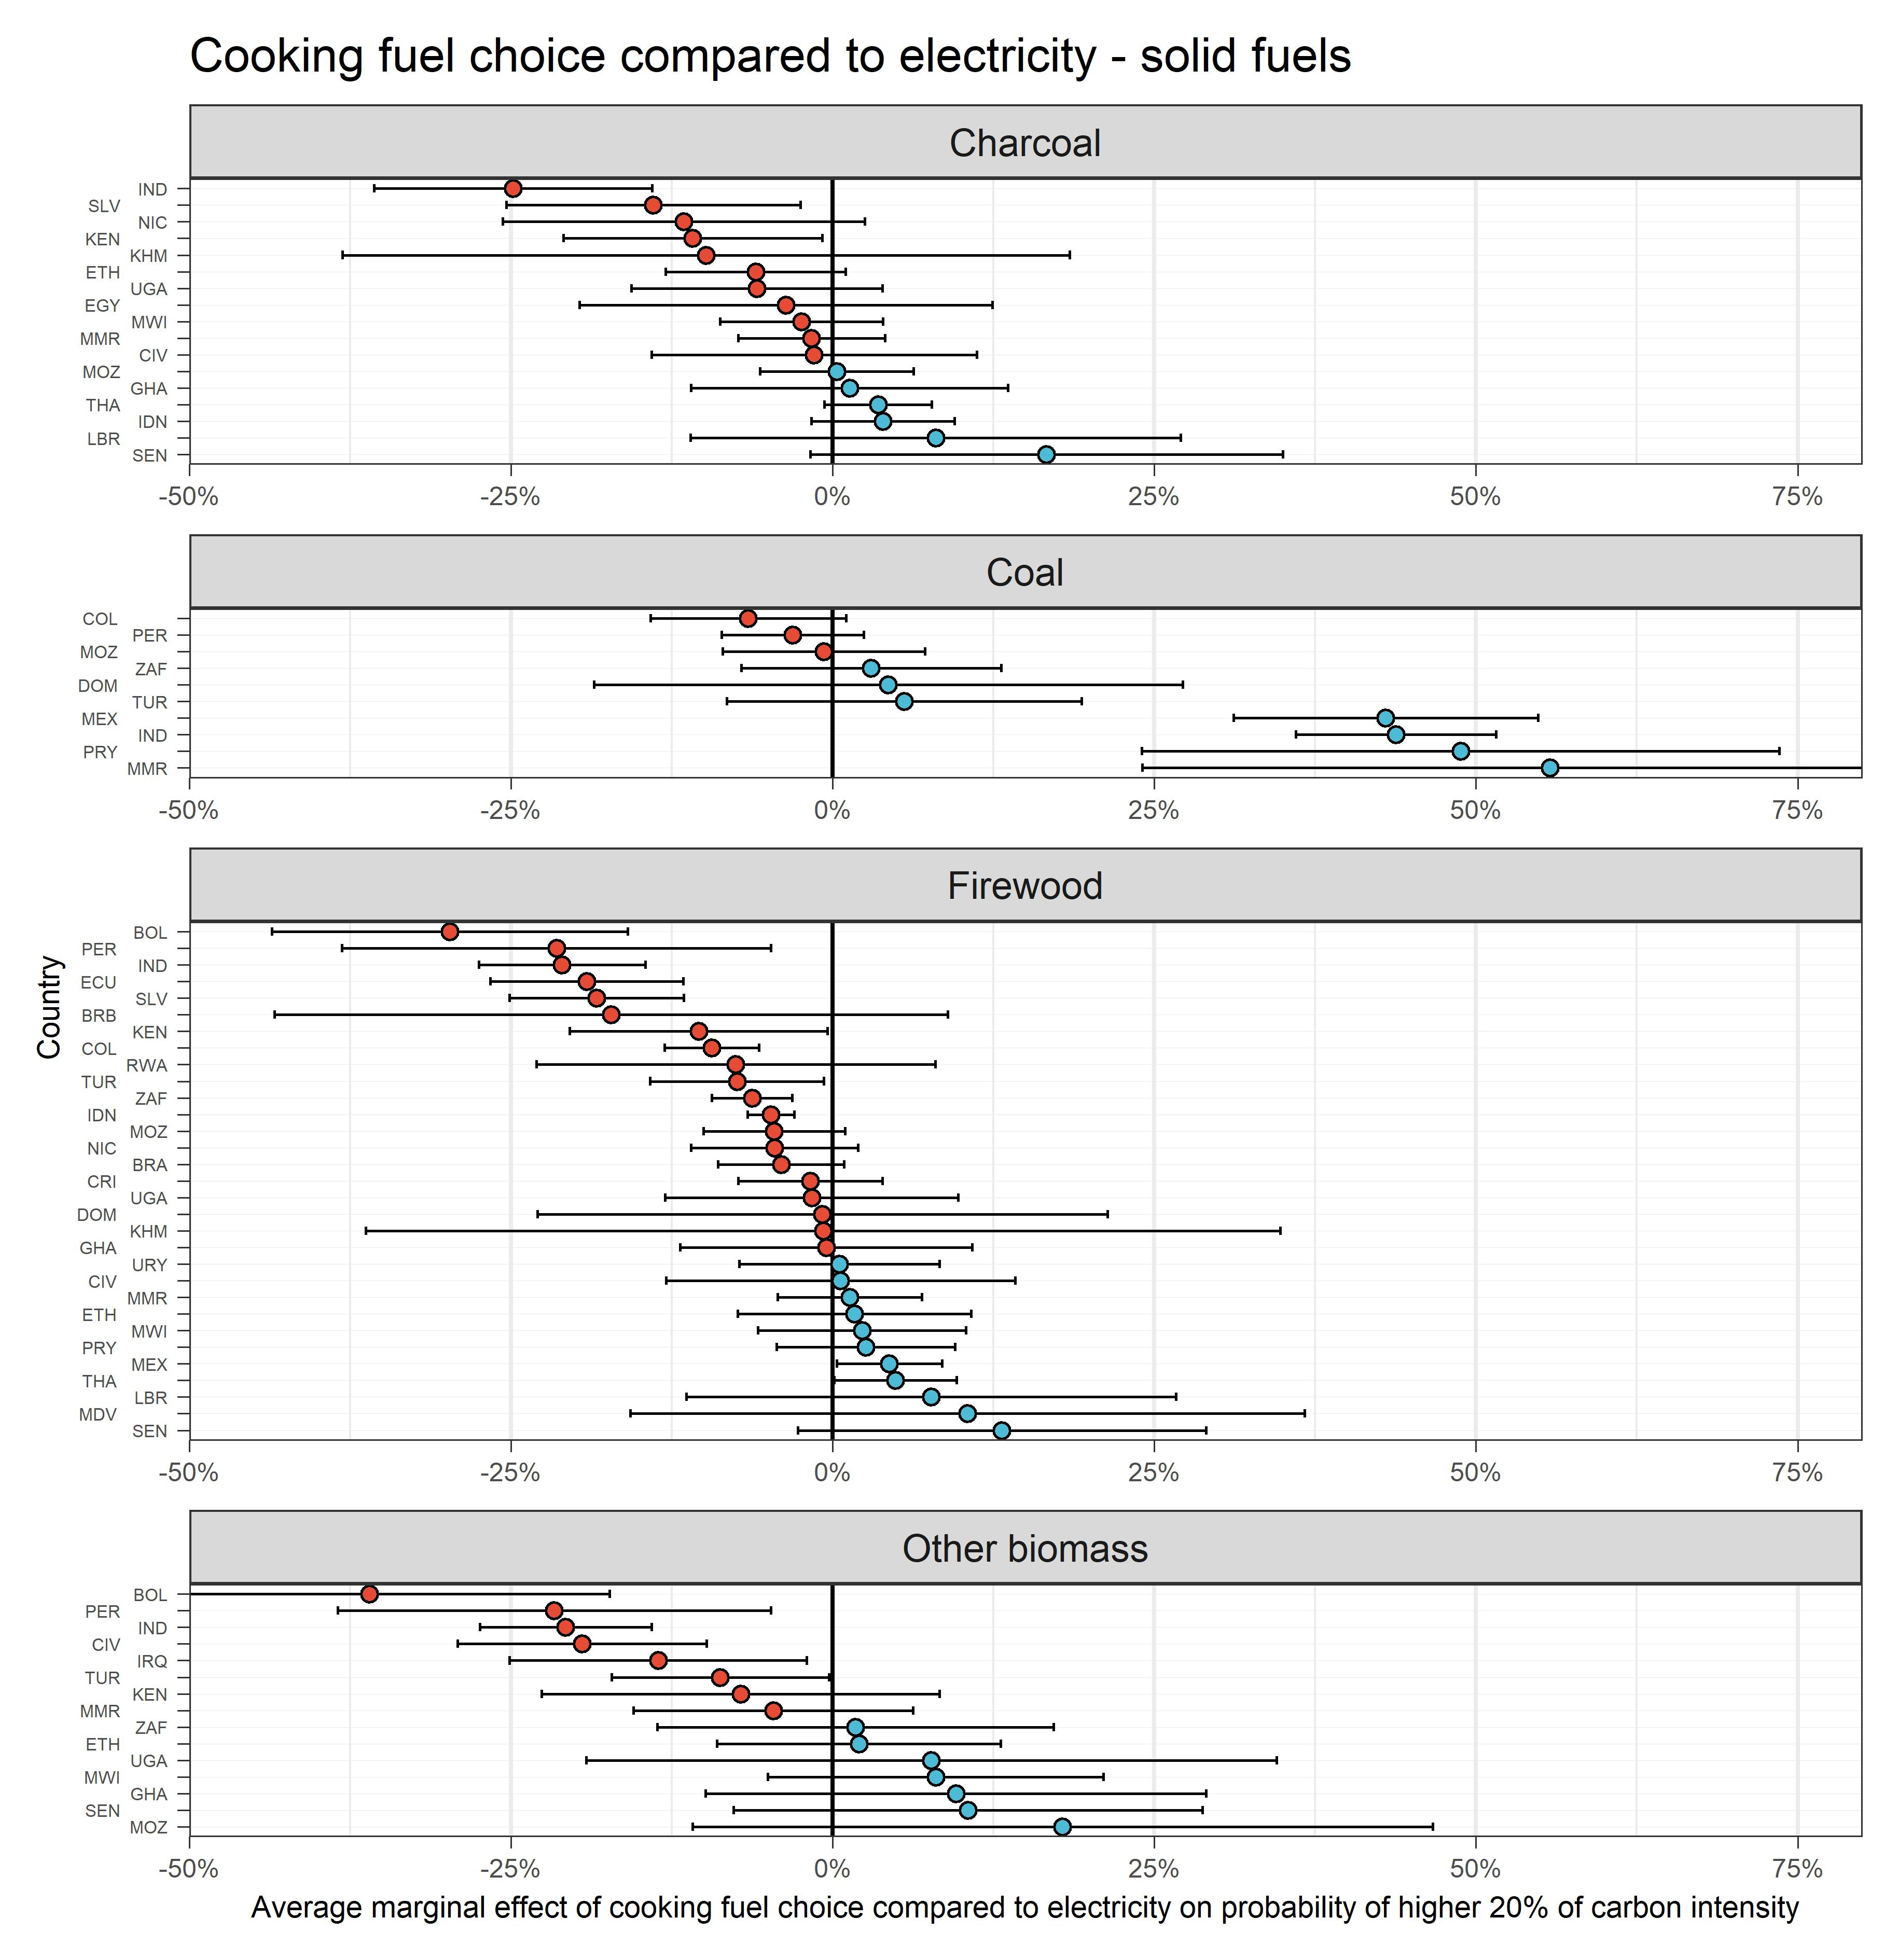
\includegraphics{1_Figures/Analysis_Logit_Models_Marginal_Effects/Average_Marginal_Effects_affected_upper_80_CF_Electricity A_2017.jpg}
   \begin{subcaption2}
     This figure shows average marginal effects of using different cooking fuels (compared to using electricity) on the probability of consuming more carbon intensively than 80\% of households in each country. Estimates come from logit-models (see equation \ref{logit}) including a rich set of control variables including total household expenditures. Control variables differ for different countries. Red points display negative estimates; blue points display positive estimates. Error bars display 95\%-confidence interval. Estimates are ordered in descending order.
   \end{subcaption2}
   \end{subfigure}
 \end{figure}
 \clearpage

 \begin{figure}[ht!]\ContinuedFloat
   \centering
   \begin{subfigure}[b]{\textwidth}
   \centering
   \caption{Average marginal effects of cooking fuel choice - part B} \label{fig:Logit_ME_CF_2}
   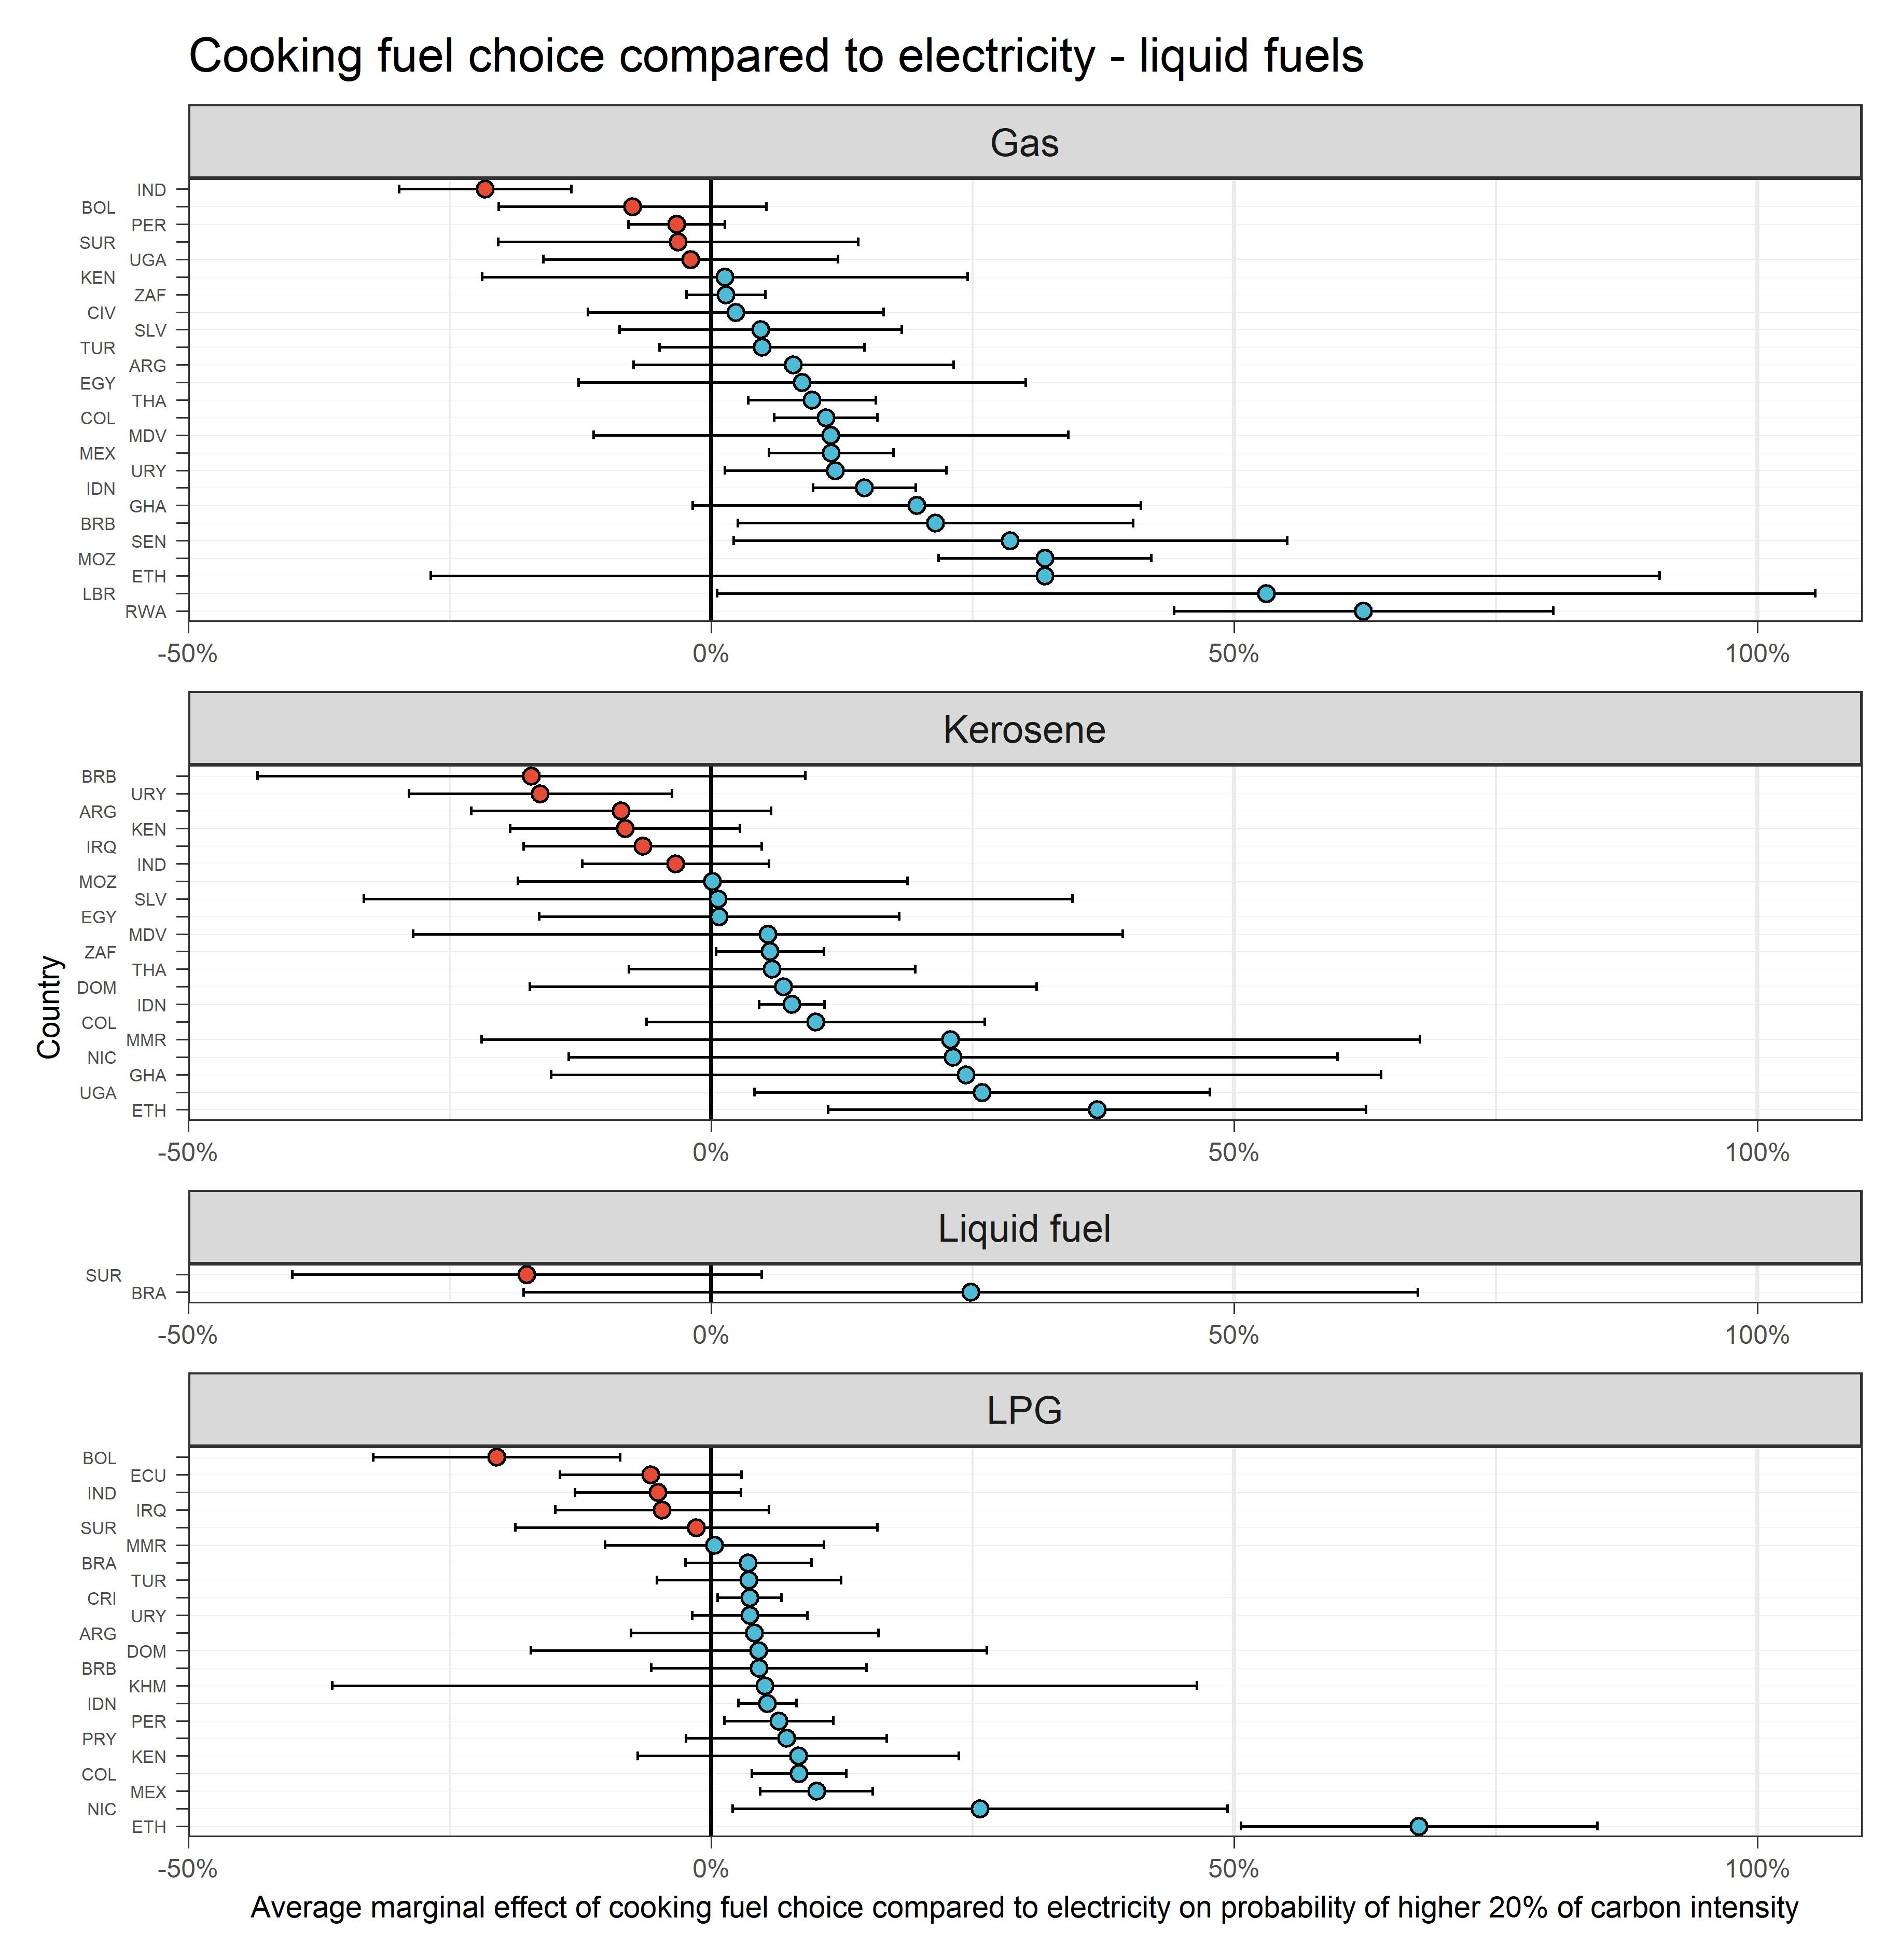
\includegraphics{1_Figures/Analysis_Logit_Models_Marginal_Effects/Average_Marginal_Effects_affected_upper_80_CF_Electricity B_2017.jpg}
   \begin{subcaption2}
     This figure shows average marginal effects of using different cooking fuels (compared to using electricity) on the probability of consuming more carbon intensively than 80\% of households in each country. Estimates come from logit-models (see equation \ref{logit}) including a rich set of control variables including total household expenditures. Control variables differ for different countries. Red points display negative estimates; blue points display positive estimates. Error bars display 95\%-confidence interval. Estimates are ordered in descending order.
   \end{subcaption2}
   \end{subfigure}
 \end{figure}
 \clearpage

 \begin{figure}[ht!]\ContinuedFloat
   \centering
   \begin{subfigure}[b]{\textwidth}
   \centering
   \caption{Average marginal effects of cooking fuel choice - part C} \label{fig:Logit_ME_CF_3}
   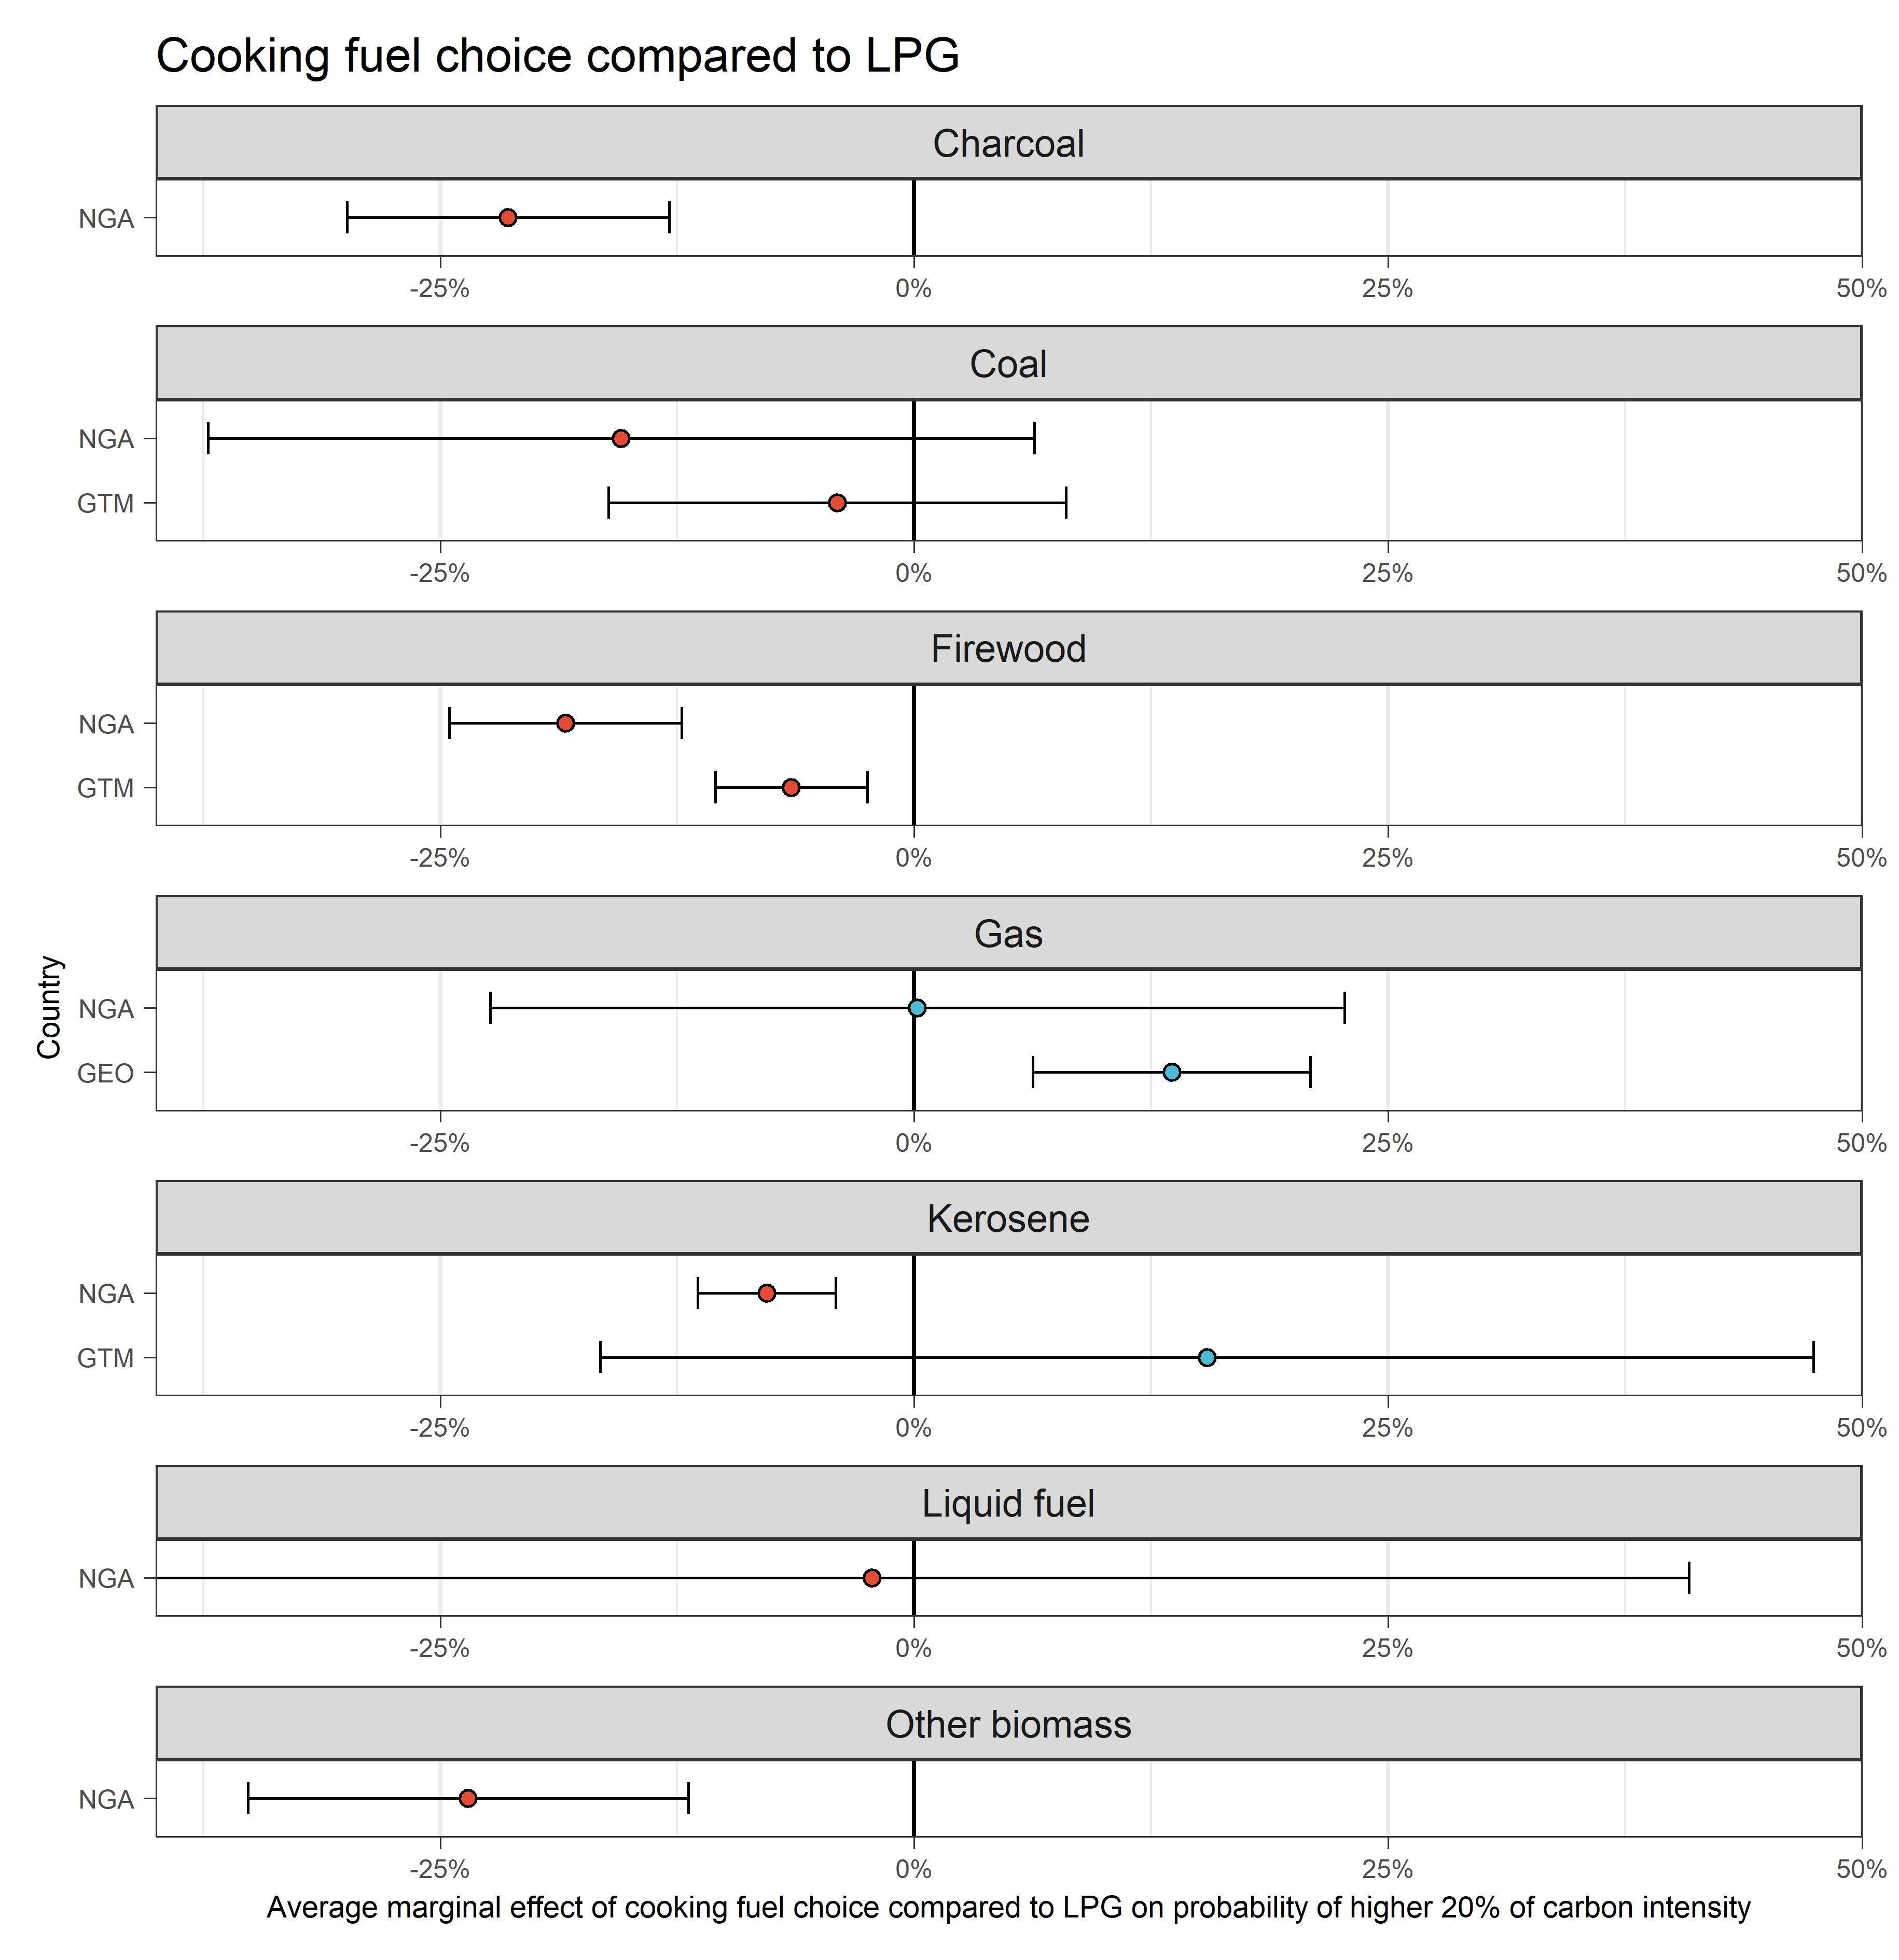
\includegraphics{1_Figures/Analysis_Logit_Models_Marginal_Effects/Average_Marginal_Effects_affected_upper_80_CF_LPG_2017.jpg}
   \begin{subcaption2}
     This figure shows average marginal effects of using different cooking fuels (compared to using LPG) on the probability of consuming more carbon intensively than 80\% of households in each country. Estimates come from logit-models (see equation \ref{logit}) including a rich set of control variables including total household expenditures. Control variables differ for different countries. Red points display negative estimates; blue points display positive estimates. Error bars display 95\%-confidence interval. Estimates are ordered in descending order.
   \end{subcaption2}
   \end{subfigure}
 \end{figure}
 \clearpage

 \begin{figure}[ht!]\ContinuedFloat
   \centering
   \begin{subfigure}[b]{\textwidth}
   \centering
   \caption{Average marginal effects of cooking fuel choice - part D} \label{fig:Logit_ME_CF_4}
   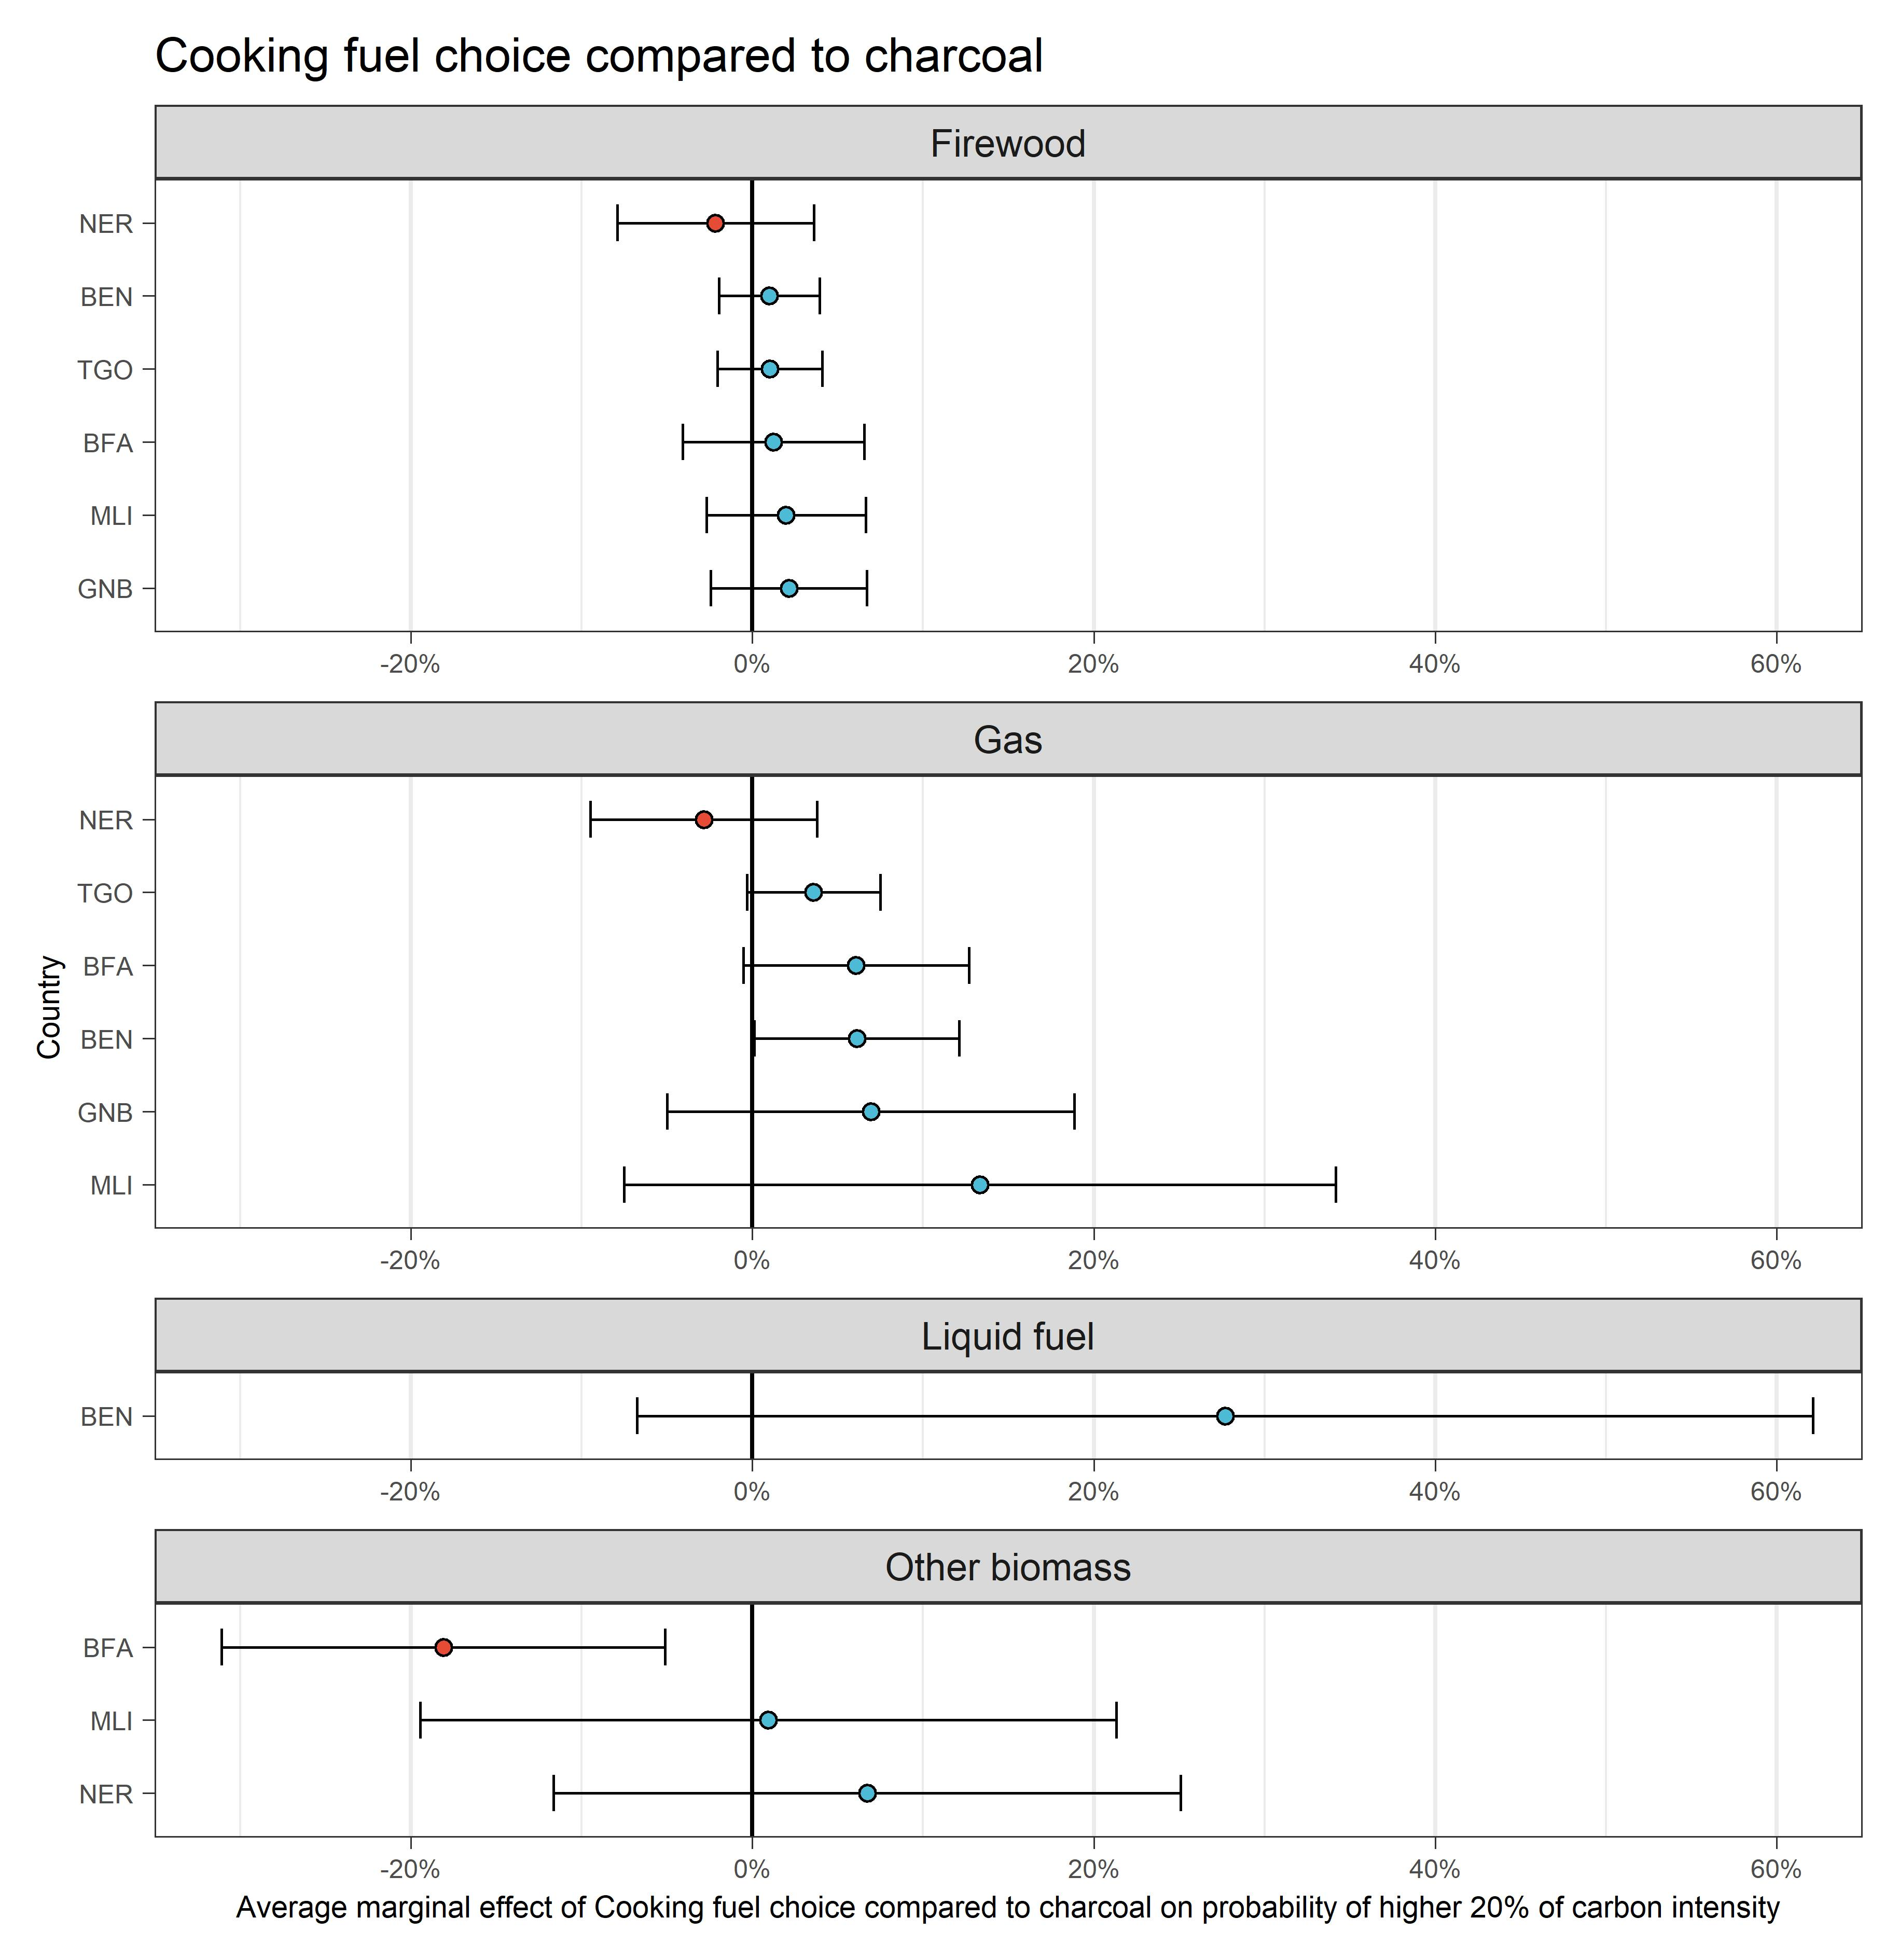
\includegraphics{1_Figures/Analysis_Logit_Models_Marginal_Effects/Average_Marginal_Effects_affected_upper_80_CF_Charcoal_2017.jpg}
   \begin{subcaption2}
     This figure shows average marginal effects of using different cooking fuels (compared to using charcoal) on the probability of consuming more carbon intensively than 80\% of households in each country. Estimates come from logit-models (see equation \ref{logit}) including a rich set of control variables including total household expenditures. Control variables differ for different countries. Red points display negative estimates; blue points display positive estimates. Error bars display 95\%-confidence interval. Estimates are ordered in descending order.
   \end{subcaption2}
   \end{subfigure}
 \end{figure}
 \clearpage
